\documentclass[lang=cn,newtx,10pt,scheme=chinese]{elegantbook}

\title{数学分析学习笔记}
\subtitle{复习整理笔记}

\author{阮炜挺}
\institute{宁波大学数学与统计学院}
\date{}

\extrainfo{Given yourself an epsilon of room!}

\setcounter{tocdepth}{3}

\cover{cover.jpg}

% 本文档命令
\usepackage{array}
\newcommand{\ccr}[1]{\makecell{{\color{#1}\rule{1cm}{1cm}}}}

% 修改标题页的橙色带
\definecolor{customcolor}{RGB}{32,178,170}
\colorlet{coverlinecolor}{customcolor}
\usepackage{cprotect}

\addbibresource[location=local]{reference.bib} % 参考文献,不要删除
\everymath{\displaystyle} % 使所有公式默认使用行间公式
\usepackage{extarrows}

\begin{document}

\maketitle
\frontmatter

\tableofcontents

\mainmatter

\chapter{含参变量积分}

\section{基本定理}

\begin{theorem}[连续性]
设 $f(x,t)$ 在 $[a,b] \times [c,d]$ 上连续, 则 $\varphi(t) = \int_{a}^{b} f(x,t) dx$ 在 $[c,d]$ 上连续, 即
$$ \lim\limits_{t \to t_0} \int_{a}^{b} f(x,t) dx = \int_{a}^{b} f(x, t_0) dx = \int_{a}^{b} \lim\limits_{t \to t_0} f(x,t) dx, \quad \forall t_0 \in [c,d]. $$
\end{theorem}

\begin{theorem}[交换积分次序]
设 $f(x,t)$ 在 $[a,b] \times [c,d]$ 上连续, 则
$$ \int_{c}^{d} dt \int_{a}^{b} f(x,t) dx = \int_{a}^{b} dx \int_{c}^{d} f(x,t) dt. $$
\end{theorem}

\begin{theorem}[可微性]
设 $f(x,t), f_t(x,t)$ 在 $[a,b] \times [c,d]$ 上连续, 则 $\varphi(t) = \int_{a}^{b} f(x,t) dx$ 在 $[c,d]$ 上可导, 且
$$ \varphi'(t) = \int_{a}^{b} f_t(x,t) dx. $$
\end{theorem}

\begin{theorem}[一般情形的连续性与可微性]
设 $f(x,t)$ 在 $[a,b] \times [c,d]$ 上连续, 函数 $\alpha(t), \beta(t)$ 在 $[c,d]$ 上连续, 且 $a \le \alpha(t), \beta(t) \le b, \forall t \in [a,b]$, 则 $\varphi(t) = \int_{\alpha(t)}^{\beta(t)} f(x,t) dx$ 在 $[c,d]$ 上连续. 进一步, 若 $f_t(x,t)$ 在 $[a,b] \times [c,d]$ 上连续, $\alpha(t), \beta(t)$ 在 $[c,d]$ 上可导, 则 $\varphi(t)$ 也在 $[c,d]$ 上可导, 且
$$ \varphi'(t) = f[\beta(t),t]\beta'(t) - f[\alpha(t),t]\alpha'(t) + \int_{\alpha(t)}^{\beta(t)} f_t(x,t) dx. $$
\end{theorem}

\section{含参变量正常积分}

\subsection{简单例题}
\begin{example}
设 $f(x,y) = \operatorname{sgn}(x-y)$, 证明: 含参量积分 $F(y) = \int_{0}^{1} f(x,y) \,dx$ 在 $(-\infty, +\infty)$ 上连续.
\end{example}
\begin{solution}
对$y$的范围进行讨论有$F(y) = \begin{cases} 1, & y < 0, \\ 1-2y, & 0 \le y \le 1, \\ -1, & y > 1. \end{cases} $ $\blacksquare$
\end{solution} 

\begin{example}
设 $x>0$, 且 $f(x) = \int_{x}^{x^2} \frac{\sin ux}{u} \,du$, 求 $f'(x)$.
\end{example}
\begin{solution}
\begin{align*}
f'(x) &= 2x \cdot \frac{\sin x^3}{x^2} - \frac{\sin x^2}{x} + \int_{x}^{x^2} \cos ux \,du = \frac{2\sin x^3 - \sin x^2}{x} + \frac{\sin ux}{x} \bigg|_{x}^{x^2} = \frac{3\sin x^3 - 2\sin x^2}{x}. \blacksquare
\end{align*}

\end{solution}

\begin{example}[$\bigstar$]
设 $f(x)$ 在 $[0,1]$ 上连续, 讨论函数 $F(t) = \int_0^1 \frac{t}{x^2+t^2}f(x)dx$ 的连续性.
\end{example}

\begin{solution}
令 $g(x,t) = \frac{t}{x^2+t^2}f(x)$, 那么 $F(t) = \int_0^1 g(x,t) dx$. 注意到 $F(t)$ 是奇函数.
$\forall t_0 \in (0, +\infty)$, $g(x,t)$ 在 $[0,1] \times [\frac{t_0}{2}, 2t_0]$ 中连续, 那么 $F(t)$ 在 $[\frac{t_0}{2}, 2t_0]$ 连续.
从而 $F(t)$ 在 $t_0$ 点连续, 从而 $F(t)$ 在 $(0, +\infty)$ 连续. 同理 $F(t)$ 在 $(-\infty, 0)$ 也连续, 故 $F(t)$ 在 $(-\infty, 0) \cup (0, +\infty)$ 连续.

接下来讨论 $t=0$ 处. 首先有 $F(0)=0$. 再考虑
$$ \lim\limits_{t \to 0^+} F(t) = \boxed{\lim\limits_{t \to 0^+} \int_0^1 \frac{t}{x^2+t^2}f(x)dx }$$
我们将积分拆分为两部分:
$$ \int_0^1 \frac{t}{x^2+t^2}f(x)dx = \int_0^{t^{\frac{1}{4}}} \frac{t}{x^2+t^2}f(x)dx + \int_{t^{\frac{1}{4}}}^1 \frac{t}{x^2+t^2}f(x)dx = I_1 + I_2 $$
\begin{enumerate}
    \item 对于 $I_1 = \int_0^{t^{\frac{1}{4}}} \frac{t}{x^2+t^2}f(x)dx$, 由积分中值定理, 存在 $\xi \in (0, t^{\frac{1}{4}})$, 使得
    $$ I_1 = f(\xi) \int_0^{t^{\frac{1}{4}}} \frac{t}{x^2+t^2}dx = f(\xi)\left[\arctan \frac{x}{t}\right]_0^{t^{\frac{1}{4}}} = f(\xi) \arctan\frac{t^{\frac{1}{4}}}{t} = f(\xi) \arctan\frac{1}{t^{\frac{3}{4}}} $$
    那么当 $t \to 0^+$ 时, $\xi \to 0$, $\arctan\frac{1}{t^{\frac{3}{4}}} \to \frac{\pi}{2}$.
    从而
    $$ \lim\limits_{t \to 0^+} I_1 = \lim\limits_{t \to 0^+} f(\xi) \arctan\frac{1}{t^{\frac{3}{4}}} = f(0) \cdot \frac{\pi}{2} $$
    \item 对于 $I_2 = \int_{t^{\frac{1}{4}}}^1 \frac{t}{x^2+t^2}f(x)dx$, 由于 $f$ 在 $[0,1]$ 上连续, 故有界, 不妨设 $|f(x)| \le M$. 那么
    $$ |I_2| \le M \int_{t^{\frac{1}{4}}}^1 \frac{t}{x^2+t^2}dx = M \left(\arctan \frac{1}{t} - \arctan \frac{t^{\frac{1}{4}}}{t}\right) = M\left(\arctan\frac{1}{t} - \arctan\frac{1}{t^{\frac{3}{4}}}\right) $$
    由于当 $t \to 0^+$ 时, $\arctan\frac{1}{t} \to \frac{\pi}{2}$ 且 $\arctan\frac{1}{t^{\frac{3}{4}}} \to \frac{\pi}{2}$, 故 $\lim\limits_{t \to 0^+} M\left(\arctan\frac{1}{t} - \arctan\frac{1}{t^{\frac{3}{4}}}\right) = 0$.
    所以 $\lim\limits_{t \to 0^+} I_2 = 0$.
\end{enumerate}
由 1 和 2 可知 $\lim\limits_{t \to 0^+} F(t) = \frac{\pi}{2}f(0) + 0 = \frac{\pi}{2}f(0)$.
因为 $F(t)$ 是奇函数, 同理可得 $\lim\limits_{t \to 0^-} F(t) = -\lim\limits_{t \to 0^+} F(-t) = -F(0^+) = -\frac{\pi}{2}f(0)$.
$F(t)$ 在 $t=0$ 处连续的充要条件是左右极限存在且等于 $F(0)=0$.
$$ \lim\limits_{t \to 0^+} F(t) = \lim\limits_{t \to 0^-} F(t) = F(0) \implies \frac{\pi}{2}f(0) = -\frac{\pi}{2}f(0) = 0 $$
这等价于 $f(0)=0$.
所以, 当 $f(0)=0$ 时, $F(t)$ 在 $t=0$ 处连续. 当 $f(0) \neq 0$ 时, $F(t)$ 在 $t=0$ 处不连续.$\hfill \blacksquare$
\end{solution}

\begin{example}
证明函数 $J(x) = \frac{1}{\pi}\int_{0}^{\pi} \cos(t - x \sin t) \,dt$ 满足
$$ x^2 J''(x) + x J'(x) + (x^2 - 1)J(x) = 0. $$
\end{example}
\begin{note}
    操作过程中用分部积分把积分中的三角函数统一名称即可,需要注意的是分部积分过程中要看清楚是对哪个变量进行求导.此题也说明有时候通过简单的四则运算并不能消去所有项,这题最后剩下了一个积分为零的项.
\end{note}

\begin{solution}
首先注意到
\begin{align*}
J'(x) &= \frac{1}{\pi} \int_{0}^{\pi} \sin(t - x\sin t)\sin t \,dt = -\frac{1}{\pi} \int_{0}^{\pi} \sin(t - x\sin t) \,d(\cos t) \\
&= -\frac{1}{\pi}\sin(t-x\sin t)\cos t \bigg|_{0}^{\pi} + \frac{1}{\pi} \int_{0}^{\pi} \cos(t - x\sin t)(1 - x\cos t)\cos t \,dt  \text{\color{red}(注意分部积分的变量是t)}\\
&= \frac{1}{\pi} \int_{0}^{\pi} \cos(t-x\sin t)\cos t \,dt - \frac{x}{\pi}\int_{0}^{\pi} \cos(t-x\sin t)\cos^2 t \,dt.
\end{align*}
另外, 还有
\begin{align*}
J''(x) &= \frac{1}{\pi} \int_{0}^{\pi} \cos(t-x\sin t)(-\sin^2 t) \,dt \\
&= \frac{1}{\pi} \int_{0}^{\pi} \cos(t-x\sin t)\cos^2 t \,dt - \frac{1}{\pi}\int_{0}^{\pi} \cos(t-x\sin t) \,dt.
\end{align*}
由此可知
\begin{align*}
x^2 J''(x) + x J'(x) + (x^2-1)J(x) = -\frac{1}{\pi}\big[\sin(t-x\sin t)\big]_{0}^{\pi} = 0.\blacksquare
\end{align*}


\end{solution}

\begin{example}
设 $f(x)$ 在 $a$ 的某邻域内具有连续的 $n+1$ 阶导函数, 求 $\lim\limits_{x \to a} \frac{d^n}{dx^n} \left[ \frac{f(x) - f(a)}{x-a} \right]$.
\end{example}

\begin{solution}
注意到 $x \neq a$ 时, 有
$$ \boxed{\frac{f(x)-f(a)}{x-a} = \int_{0}^{1} f'(a+t(x-a)) \,dt}. $$
因此
$$ \frac{d^n}{dx^n} \left[ \frac{f(x)-f(a)}{x-a} \right] = \int_{0}^{1} f^{(n+1)}(a+t(x-a))\cdot t^n \,dt. $$
再结合 $f^{(n+1)}(x)$ 的\underline{连续性}, 有
$$ \lim\limits_{x \to a} \frac{d^n}{dx^n} \left[ \frac{f(x)-f(a)}{x-a} \right] = \int_{0}^{1} \lim\limits_{x \to a} \left\{ f^{(n+1)}[a+t(x-a)] \cdot t^n \right\} dt = f^{(n+1)}(a) \int_{0}^{1} t^n \,dt = \frac{f^{(n+1)}(a)}{n+1}. $$
\hfill $\blacksquare$
\end{solution}

\begin{example}
设 $F(t) = \int_{0}^{t} dx \int_{x^2}^{t^2} f(x,y) \,dy$, 其中 $f(x,y)$ 为连续函数, 求 $F'(t)$.
\end{example}

\begin{solution}
即定理1.4的应用.
记 $g(x,t) = \int_{x^2}^{t^2} f(x,y) \,dy$, 则 $F(t) = \int_{0}^{t} g(x,t) \,dx$,又因为$g_t(x,t) = f(x,t^2)\cdot 2t + \int_{x^2}^{t^2} f_t(x,y)dy = 2tf(x,t^2)$,
从而有$F'(t) = g(t,t)+\int_{0}^{t}g_t(x,t)dx = \int_{0}^{t}2tf(x,t^2)dx$ $blacksquare$.
\end{solution}
\begin{note}
    累次含参变量积分的处理方法,通过设 $g(x,t)$ 为积分的被积函数, 来化为一般形式的含参变量积分.
\end{note}

\begin{example}
设 $F(t) = \int_0^a dx \int_0^a f(x+y+t) dy$, 其中 $f$ 为连续函数. 证明
$$F''(t) = f(t+2a) - 2f(t+a) + f(t).$$
\end{example}

\begin{solution}
由于 $f$ 只是连续函数, 故不能直接对积分号下的 $f$ 求二阶导数.
令 $g(x,t) = \int_0^a f(x+y+t) dy$, 从而 $F(t) = \int_0^a g(x,t) dx$.
不妨设 $f$ 的原函数为 $H$, $H$ 的原函数为 $G$. (即 $H'=f, G'=H, G''=f$)
那么
$$ g(x,t) = \int_0^a f(x+y+t) dy = \big[ H(x+y+t) \big]_{y=0}^{y=a} = H(x+t+a) - H(x+t). $$
而
\begin{align*}
F(t) &= \int_0^a g(x,t) dx = \int_0^a [H(x+t+a) - H(x+t)] dx \\
&= \big[ G(x+t+a) \big]_{x=0}^{x=a} - \big[ G(x+t) \big]_{x=0}^{x=a} \\
&= [G(a+t+a) - G(0+t+a)] - [G(a+t) - G(0+t)] \\
&= G(t+2a) - G(t+a) - G(t+a) + G(t) \\
&= G(t+2a) - 2G(t+a) + G(t).
\end{align*}
那么
$$ F''(t) = \frac{d^2}{dt^2} [G(t+2a) - 2G(t+a) + G(t)] = G''(t+2a) - 2G''(t+a) + G''(t). $$
因为 $G''=f$, 所以
$$ F''(t) = f(t+2a) - 2f(t+a) + f(t) \blacksquare$$
\end{solution}

\begin{example}[$\bigstar$]
计算累次积分 $\int_0^1 dx \int_0^1 \frac{x^2 - y^2}{(x^2 + y^2)^2} dy$ 与  $\int_0^1 dy \int_0^1 \frac{x^2 - y^2}{(x^2 + y^2)^2} dx$.
\end{example}

\begin{solution}
    令$$P(x,y) = \frac{x}{(x^2 + y^2)}, Q(x,y) = \frac{y}{(x^2 + y^2)}$$ 注意到$$P_x(x,y) = \frac{y^2 - x^2}{(x^2 + y^2)^2}, Q_y(x,y) = \frac{x^2 - y^2}{(x^2 + y^2)^2}$$
    且有$-P_x(x,y) = Q_y(x,y)$

    那么
    $$
    \int_0^1 dx \int_0^1 \frac{x^2 - y^2}{(x^2 + y^2)^2} dy = \int_0^1 dx \int_0^1 Q_y(x,y) dy = \int_0^1 Q(x,y) \bigg|_{y=0}^{y=1} dx = \int_0^1 \frac{1}{1+x^2} dx = \frac{\pi}{4}.
    $$
    同理
    $$
    \int_0^1 dy \int_0^1 \frac{x^2 - y^2}{(x^2 + y^2)^2} dx = \int_0^1 dy \int_0^1 -P_x(x,y) dx = \int_0^1 -P(x,y) \bigg|_{x=0}^{x=1} dy = -\int_0^1 \frac{1}{1+y^2} dy = -\frac{\pi}{4}.
    $$
    $\hfill \blacksquare$
\end{solution}

\subsection{含参变量积分的计算}
\begin{proposition}
当 $|a|<1$ 时, 有
\begin{equation*}
\int \frac{dx}{1+a\cos x} = \frac{2}{\sqrt{1-a^2}} \arctan\left(\sqrt{\frac{1-a}{1+a}}\tan\frac{x}{2}\right) + C. 
\end{equation*}

特别地, 有
\begin{equation*}
\int_{0}^{\pi} \frac{dx}{1+a\cos x} = \frac{\pi}{\sqrt{1-a^2}}, \quad |a|<1. 
\end{equation*}
类似的还有
$$
\int_{0}^{\pi} \frac{1}{a + \cos x} dx = \frac{\pi}{\sqrt{a^2 - 1}}, \quad a > 1.
$$

$$
\int_{0}^{\pi} \frac{1}{a + \cos x} dx =  - \frac{\pi}{\sqrt{a^2 - 1}}, \quad a < 1.
$$
\end{proposition}
\begin{remark}
    此命题用万能公式即可.
\end{remark}

如果直接求$\varphi(t) = \int_{a}^{b}f(x,t) \mathrm d x$有困难,那么通常采用以下两种方法:
\textcolor{blue}{\begin{enumerate}
    \item \textbf{积分号下积分}:把$f(x,t)$表示为积分形式,再用积分号下求积分的方法,此时通常要交换积分次序,所以要先判断函数的连续性.
    \item \textbf{积分号下微分}:先求$\varphi'(t)$,即先求$\int_{a}^{b}f_t(x,t) \mathrm d x$,然后再对$t$积分求出$\varphi(t)$,所以要先判断$f(x,t)$和$f_t(x,t)$的连续性.
\end{enumerate}}

\subsubsection{积分号下积分}

\begin{example}
计算 $\int_0^1 \frac{x^b - x^a}{\ln x} dx$, 其中 $0 < a < b$.
\end{example}

\begin{solution}
注意到 $$\frac{x^b - x^a}{\ln x} = \left[ \frac{x^y}{\ln x} \right]_{y=a}^{y=b} = \int_a^b x^y dy$$
那么
\begin{align*}
\int_0^1 \frac{x^b - x^a}{\ln x} dx &= \int_0^1 dx \int_a^b x^y dy \quad (\text{由于 } x^y \text{ 在 } [0,1] \times [a,b] \text{ 上连续, 故可交换积分次序}) \\
&= \int_a^b dy \int_0^1 x^y dx = \int_a^b \left[ \frac{x^{y+1}}{y+1} \right]_{x=0}^{x=1} dy = \int_a^b \frac{1}{y+1} dy \\
&= \big[ \ln(y+1) \big]_{y=a}^{y=b} = \ln(b+1) - \ln(a+1) = \ln\frac{b+1}{a+1}. 
\end{align*}
$ \hfill \blacksquare$
\end{solution}

\begin{example}
计算 $\int_0^1 \sin\left(\ln\frac{1}{x}\right)\frac{x^b - x^a}{\ln x}dx$ 与 $\int_0^1 \cos\left(\ln\frac{1}{x}\right)\frac{x^b - x^a}{\ln x}dx$, 其中 $0 < a < b$.
\end{example}

\begin{solution}
注意到 $\frac{x^b - x^a}{\ln x} = \int_a^b x^y dy$, 那么$\int_0^1 \sin\left(\ln\frac{1}{x}\right)\frac{x^b - x^a}{\ln x}dx = \int_0^1dx\int_a^b x^y\sin(\ln\frac 1 x)dy$,

令$f(x,y) = x^y\sin(\ln\frac 1 x)$, 且有$\lim_{x \to 0^+} f(x,y) = 0,\forall y \in [a,b]$,那么可以令
$$F(y) = \begin {cases}
 x^y\sin(\ln\frac 1 x),&0< x \leq 1 \\
    0,  &x = 0.
\end{cases}$$
从而$F(x,y)$在$[0,1] \times [a,b]$ 上连续, 故积分可以交换次序, 从而有
$$
\int_0^1 \sin\left(\ln\frac{1}{x}\right)\frac{x^b - x^a}{\ln x}dx =\int_0^1 dx \int_a^b f(x,y) dy =\int_{0}^{1} dx \int_{a}^{b} F(x,y) dy = \int_a^b dy \int_0^1 F(x,y) dx = \int_a^b dy \int_0^1 x^y \sin(\ln\frac{1}{x}) dx
$$
令$u = \ln \frac{1}{x}$,那么上式可化为
$$\int_a^b dy \int_0^{+\infty} e^{-u} e^{-yu} \sin u \,du = \int_a^b dy \int_0^{+\infty} e^{-(y+1)u} \sin u \,du$$
\begin{figure}[h]
	\centering 
	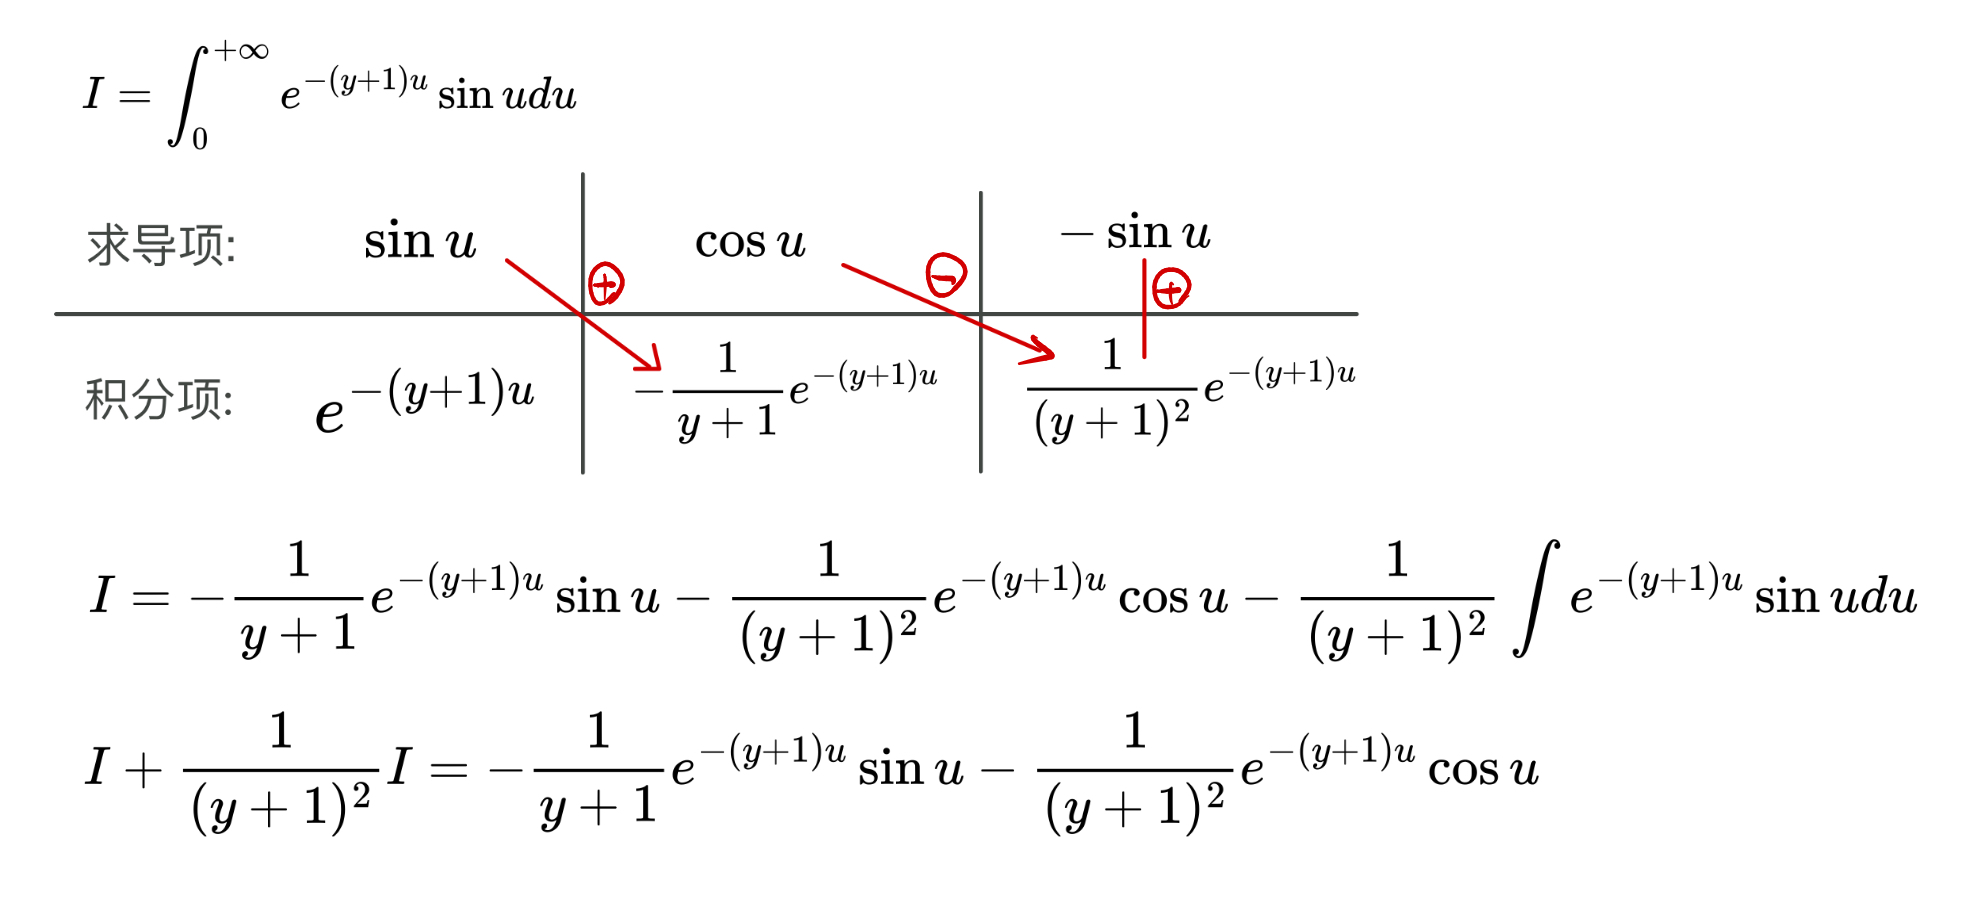
\includegraphics[width=0.9\textwidth]{表格法1.jpg} 
\end{figure}

右边将上下限代入即得
$$\int_0^1 \sin\left(\ln\frac{1}{x}\right)\frac{x^b - x^a}{\ln x}dx = \int_a^b \frac{1}{(y+1)^2 + 1} dy = \arctan(b+1) - \arctan(a+1).$$

同理可得
\begin{align*}
    \int_0^1 \cos\left(\ln\frac{1}{x}\right)\frac{x^b - x^a}{\ln x}dx &= \int_a^b dy \int_0^{+\infty} e^{-(y+1)u} \cos u \,du = \int_{a}^{b} \frac{y+1}{(y+1)^2 +1}dy \\
&= \frac{1}{2} \ln\left((y+1)^2 + 1\right) \bigg|_{y=a}^{y=b} =  \frac 1 2 \ln\frac{(b+1)^2 + 1}{(a+1)^2 + 1}. \blacksquare
\end{align*}
\end{solution}

\begin{example}
计算 $F(\alpha) = \int_{0}^{\frac{\pi}{2}} \ln\frac{1+\alpha\cos x}{1-\alpha\cos x} \cdot \frac{1}{\cos x}dx$, 其中 $\alpha \in (-1,1)$.
\end{example}

\begin{solution}
$$ F(\alpha) = \int_0^{\frac{\pi}{2}} \frac{\ln(1+\alpha\cos x) - \ln(1-\alpha\cos x)}{\cos x} dx =\int_0^{\frac{\pi}{2}} dx \int_{-\alpha}^{\alpha} \frac{1}{1+y\cos x} dy $$
此时, 令 $f(x,y) = \frac{1}{1+y\cos x}$, 该函数在区域 $[0, \frac{\pi}{2}] \times [-\alpha, \alpha]$ 上连续. 故积分次序可交换.
\begin{note}
    寻找函数的过程:
    
    积分里是$\frac{\ln(1+\alpha\cos x) - \ln(1-\alpha\cos x)}{\cos x}=\frac{\ln(1+y\cos x)}{\cos x}\bigg|_{y=-\alpha}^{y=\alpha}$,那么对$\frac{\ln(1+y\cos x)}{\cos x}$关于$y$求导即可得积分中的被积函数,在此例中求导后得到的就是$\frac{1}{1+y\cos x}$
\end{note}

\begin{align*}
\int_0^{\frac{\pi}{2}} dx \int_{-\alpha}^\alpha \frac{1}{1+y\cos x} dy &
= \int_{-\alpha}^\alpha dy \int_0^{\frac{\pi}{2}} \frac{1}{1+y\cos x} dx \\
& = \color{blue}{\boxed{\int_{-\alpha}^0 dy \int_0^{\frac{\pi}{2}} \frac{dx}{1+y\cos x} + \int_0^\alpha dy \int_0^{\frac{\pi}{2}} \frac{dx}{1+y\cos x}}} \color{red}{\text{(利用对称性)}}\\
& = \int_0^\alpha dy \int_0^{\frac{\pi}{2}} \frac{dx}{1-y\cos x} + \int_0^\alpha dy \int_0^{\frac{\pi}{2}} \frac{dx}{1+y\cos x} \\
& = \int_0^\alpha dy \int_0^{\frac{\pi}{2}} \frac{2dx}{1-y^2\cos^2 x} = \int_0^\alpha dy \int_0^{\frac{\pi}{2}} \frac{2\sec^2 x dx}{\tan^2 x + (1-y^2)} \\
& = \int_0^\alpha dy \int_0^{\frac{\pi}{2}} \frac{2}{\tan^2 x + (1-y^2)} d(\tan x) = \int_0^\alpha \frac{2}{\sqrt{1-y^2}} \arctan \frac{\tan x}{\sqrt{1-y^2}} \bigg|_0^{\frac{\pi}{2}} dy \\
& = \pi \int_0^\alpha \frac{dy}{\sqrt{1-y^2}} = \pi \arcsin \alpha, \quad \alpha \in (-1,1)
\end{align*}
$\hfill \blacksquare$
\end{solution}

\subsubsection{积分号下微分}
我们先来证明欧拉积分:
\begin{proposition}[欧拉积分]
$$I = \int_0^{\frac{\pi}{2}} \ln \cos t \, dt =I = \int_0^{\frac{\pi}{2}} \ln \sin u \, du = -\frac{\pi}{2}\ln 2$$
\end{proposition}

\begin{proof}
    考虑 $I = \int_0^{\frac{\pi}{2}} \ln \cos t \, dt$
    令 $u = \frac{\pi}{2} - t$, 则 $I = \int_0^{\frac{\pi}{2}} \ln \sin u \, du$
    将上面两式子相加有:
    $$2I = \int_0^{\frac{\pi}{2}} (\ln \cos t + \ln \sin t) \, dt = \int_0^{\frac{\pi}{2}} \ln (\frac{1}{2} \sin 2t) \, dt = -\frac{\pi}{2}\ln 2 + \int_0^{\frac{\pi}{2}} \ln (\sin 2t) \, dt$$
    令 $u = 2t$, 则积分变为 
    \begin{align*}
    \int_0^{\frac{\pi}{2}} \ln (\sin 2t) \, dt &= \frac{1}{2} \int_0^\pi \ln \sin u \, du =  \frac{1}{2} \int_0^{\frac{\pi}{2}} \ln \sin u \, du + \frac{1}{2} \int_{\frac{\pi}{2}}^{\pi} \ln \sin u \, du (\text{第二个积分中令}v = \frac{\pi}{2}- u)\\
     &=  \frac{1}{2} \int_0^{\frac{\pi}{2}} \ln \sin u \, du + \frac{1}{2} \int_{0}^{\frac{\pi}{2}} \ln \cos v \, dv =\frac{1}{2} \cdot 2I = I
    \end{align*}
    那么 $2I = -\frac{\pi}{2}\ln 2 + I \Rightarrow I = -\frac{\pi}{2}\ln 2$ $\hfill \blacksquare$
\end{proof}


\begin{example}[$\bigstar$]{\label{ex:integral-parameter_1}}
    计算$F(\theta)= \int_{0}^{\pi} \ln (1+\theta \cos x) \mathrm{d} x$,其中$\theta \in [-1,1]$.
\end{example}

\begin{solution}
令$f(x, \theta) = \ln(1+\theta \cos x)$, 其中$\theta \in [-1, 1]$. 注意到当$\theta = \pm 1$时, $f(x, \theta)$可能无界. 先对这两种情形讨论.
$1^\circ \theta = \pm 1$时
$$F(1) = \int_{0}^{\pi} \ln(1+\cos x)dx = \int_{0}^{\pi} \ln(2\cos^2\frac{x}{2})dx = \pi\ln2 + 2\int_{0}^{\pi}\ln(\cos\frac{x}{2})dx$$$$= \pi\ln2 + 4\int_{0}^{\pi}\ln(\cos\frac{x}{2})d(\frac{x}{2}) = \pi\ln2 + 4\int_{0}^{\frac{\pi}{2}}\ln\cos x dx = \pi\ln2 - 4 \times \frac{\pi}{2}\ln2$$$$= -\pi\ln2$$
同理$F(-1) = \int_{0}^{\pi} \ln(1-\cos x)dx = \pi\ln2 + 4\int_{0}^{\frac{\pi}{2}}\ln\sin x dx = -\pi\ln2$

$2^\circ$ 当$\theta \in (-1, 1)$时
$f'_{\theta}(x, \theta) = \frac{\cos x}{1+\theta \cos x}$, 那么此时$f(x, \theta), f'_{\theta}(x, \theta)$在$[0, \pi] \times (-1, 1)$均连续, 那么$F(\theta)$在$(-1, 1)$可导.
又因为
\begin{equation*}
F(-\theta) = \int_{0}^{\pi} \ln(1-\theta\cos x)dx \xlongequal{t=\pi-x} \int_{0}^{\pi} \ln(1+\theta\cos t)dt = F(\theta)
\end{equation*}

从而$F(\theta)$为偶函数, 那样就先求它在$(x, \theta) \in [0, \pi] \times [0, 1)$上的情形.
考虑
\begin{align*}
    F'(\theta) &= \int_{0}^{\pi} \frac{\cos x}{1+\theta \cos x}dx = \color{blue}{\frac{1}{\theta}\int_{0}^{\pi}\frac{1+\theta\cos x - 1}{1+\theta\cos x}dx} = \frac{1}{\theta}\int_{0}^{\pi}(1-\frac{1}{1+\theta\cos x})dx \\
               &= \frac{\pi}{\theta} - \frac{1}{\theta}\int_{0}^{\pi}\frac{1}{1+\theta\cos x}dx = \frac{\pi}{\theta} - \frac{\pi}{\theta\sqrt{1-\theta^2}}, |\theta|<1
\end{align*}


那么
\begin{align*}
    F(\theta)&=\int(\frac{\pi}{\theta}-\frac{\pi}{\theta\sqrt{1-\theta^2}})d\theta = \pi\ln\theta - \pi\int\frac{1}{\theta\sqrt{1-\theta^2}}d\theta+C =\pi \ln \theta - \color{blue}{\int\frac{\theta^{-2}\pi}{\sqrt{\theta^{-2}-1}}\mathrm{d} \theta +C}\\
             &=\pi \ln \theta + \int\frac{\pi}{\sqrt{\theta^{-2}-1}}\mathrm{d} \theta^{-1} +C = \pi \ln \theta +\pi \ln(\theta^{-1}+\sqrt{\theta^{-2}-1})+C=\pi \ln (1+ \sqrt{1-\theta^2}) +C
\end{align*}

当$\theta=0, F(0)=\lim\limits_{\theta \to 0} F(\theta) = \pi\ln2+C$, 而$F(0)=0$, 故$C=-\pi\ln2$.
那么$F(\theta)=\pi\ln\frac{1+\sqrt{1-\theta^2}}{2}$, 此时$F(\theta)$为偶函数.
那么在$(-1, 1)$上,$F(\theta)=\pi\ln\frac{1+\sqrt{1-\theta^2}}{2}$.

综上由$1^\circ, 2^\circ$得$F(\theta)=\pi\ln\frac{1+\sqrt{1-\theta^2}}{2}, \theta \in [-1, 1]$.
$\hfill \blacksquare$
\end{solution}

\begin{note}
    与本题类似的还有
        先计算含参变量积分$$I(\alpha) = \int _0^{\pi} \ln(\alpha +\cos x)dx,\alpha > 1$$
    易知$f(\alpha,x)$可导,且
    $$ I'(\alpha) = \int_{0}^{\pi} \frac{1}{\alpha + \cos x} dx \stackrel{t=\tan\frac{x}{2}}{=} \int_{0}^{+\infty} \frac{1}{\alpha + \frac{1-t^2}{1+t^2}} \cdot \frac{2 dt}{1+t^2}  = 2 \int_{0}^{+\infty} \frac{dt}{\alpha(1+t^2) + 1-t^2} = 2 \int_{0}^{+\infty} \frac{dt}{\alpha+1 + (\alpha-1)t^2} $$
    $$ = \frac{2}{\sqrt{\alpha^2-1}} \int_{0}^{+\infty} \frac{1}{1 + \left(\sqrt{\frac{\alpha-1}{\alpha+1}}t\right)^2} d\left(\sqrt{\frac{\alpha-1}{\alpha+1}}t\right)  = \frac{2}{\sqrt{\alpha^2-1}} \left( \arctan \sqrt{\frac{\alpha-1}{\alpha+1}}t \right) \Bigg|_{0}^{+\infty} = \frac{2}{\sqrt{\alpha^2-1}} \cdot \frac{\pi}{2} = \frac{\pi}{\sqrt{\alpha^2-1}} $$
    那么$I(\alpha) = \pi ln(\alpha +\sqrt{\alpha^2 -1})+C$,且$I(1)=\pi ln(1+0)+C=C$.

    而$I(1) = -\pi\ln 2$(降次加欧拉积分即可得).那么$C = I(1) = -\pi \ln 2$,则
    $$I(\alpha) = \pi ln(\alpha +\sqrt{\alpha^2 -1})+C= \pi ln(\alpha +\sqrt{\alpha^2 -1})-\pi \ln 2=\pi \ln \frac{\alpha+\sqrt{\alpha^2 -1}}{2}  $$$\hfill \blacksquare$
\end{note}

\begin{example}[$\bigstar$]
    计算$F(a) = \int_0^{\pi} \ln(a^2 -2a \cos x +1) \mathrm{d} x$.
\end{example}

\begin{solution}[解法1]


\begin{remark}
考虑$a^2-2a\cos x+1$, 视为$a$的二次函数.
有$\Delta=4\cos^2x-4 \le 0$. 则$\Delta < 0$时, $f(x,a)=\ln(a^2-2a\cos x+1)$有意义.
当$\Delta=0$, 即$\cos^2x=1$, 即$\cos x=\pm 1$时, $f(x,a)=\ln(a\mp 1)^2$可能无意义.
此时需对$a=\pm 1$进行讨论.
\end{remark}

$1^\circ$ 当$a=\pm 1$时
$F(1) = \int_{0}^{\pi}\ln(1-2\cos x+1)dx = \int_{0}^{\pi}(\ln 2+\ln(1-\cos x))dx = \pi\ln2 - \pi\ln2=0$,
同理有$F(-1) = \int_{0}^{\pi}\ln(1+2\cos x+1)dx=0$

$2^\circ$ 当$|a|<1$时. $F(-a)=F(a)$. 故先考虑$0<a<1$.
$f_a(x,a) = \frac{2a-2\cos x}{a^2-2a\cos x+1}$,由于$f(x,a)$,$f_a(x,a)$在$[0,\pi] \times (0,1)$上连续, 故可以求导.
即有$F'(a)=\int_{0}^{\pi}\frac{2a-2\cos x}{a^2-2a\cos x+1}dx$

\begin{align*}
    F'(a) &= \color{blue}{\frac{1}{a}\int_{0}^{\pi}\frac{a^2-2a\cos x+1-(1-a^2)}{a^2-2a\cos x+1}dx = \frac{1}{a}\int_{0}^{\pi}(1-\frac{1-a^2}{a^2-2a\cos x+1})dx}\\
          &= \frac{\pi}{a} - \frac{1-a^2}{a}\int_{0}^{\pi}\frac{1}{a^2+1-2a\cos x}dx = \frac{\pi}{a} - \frac{1-a^2}{a(1+a^2)}\int_{0}^{\pi}\frac{1}{1-\frac{2a}{1+a^2}\cos x}dx \\
          &= \frac{\pi}{a} - \frac{1-a^2}{a(1+a^2)}\frac{\pi}{\sqrt{1-(\frac{2a}{1+a^2})^2}} = \frac{\pi}{a} - \frac{1-a^2}{a(1+a^2)}\frac{\pi(a^2+1)}{|a^2-1|} = \frac{\pi}{a} - \frac{\pi}{a}\cdot\frac{1-a^2}{1-a^2} = 0
\end{align*}

从而$F(a)=C$. 又由$F(0)=0$, 而$\lim\limits_{a\to 0}F(a)=0$, 故$C=0$, 那么$F(a)=0$.
且$F(a)$为偶函数, 那么当$-1<a<1$时, $F(a)=0$.

$3^\circ$ 当$|a|>1$时, $|\frac{1}{a}|<1$,那么有

\begin{align*}
F(\frac{1}{a}) &= \int_{0}^{\pi}\ln\left(\frac{1}{a^2}-\frac{2\cos x}{a}+1\right)dx = \int_{0}^{\pi}\ln\frac{1-2a\cos x+a^2}{a^2}dx \\
&= \int_{0}^{\pi}\ln(1-2a\cos x+a^2)dx - 2\pi\ln|a| = F(a)-2\pi\ln|a|
\end{align*}

又由于$F(\frac{1}{a}) = 0 $,故 $F(a) = \begin{cases} 2\pi\ln|a|, & |a| \geq  1 \\ 0, & |a|<  1 \end{cases}$
$\hfill \blacksquare$
\end{solution}

\begin{solution}[解法2]
\begin{align*}
F(a) &= \int_{0}^{\pi} \ln(a^2 - 2a\cos x + 1)dx = \int_{0}^{\pi} \ln(a^2+1-2a\cos x)dx \\
&= \int_{0}^{\pi} \ln\left((a^2+1)\left(1-\frac{2a}{a^2+1}\cos x\right)\right)dx = \int_{0}^{\pi}\ln(a^2+1)dx + \int_{0}^{\pi}\ln\left(1-\frac{2a}{a^2+1}\cos x\right)dx \\
&= \pi\ln(a^2+1) + \int_{0}^{\pi}\ln\left(1-\frac{2a}{a^2+1}\cos x\right)dx, \quad \text{由于 } |\frac{2a}{a^2+1}| \le 1, \text{再利用上题结论} \\
&= \pi\ln(a^2+1) + \pi\ln\frac{1+\sqrt{1-\left(\frac{2a}{a^2+1}\right)^2}}{2} = \pi\ln\frac{a^2+1}{2} + \pi\ln\left(1+\sqrt{1-\frac{4a^2}{(a^2+1)^2}}\right) \\
&= \pi\ln\frac{a^2+1}{2} + \pi\ln\left(1+\sqrt{\frac{a^4+2a^2+1-4a^2}{(a^2+1)^2}}\right) = \pi\ln\frac{a^2+1}{2} + \pi\ln\left(1+\sqrt{\frac{(a^2-1)^2}{(a^2+1)^2}}\right) \\
&= \pi\ln\frac{a^2+1}{2} + \pi\ln\left(1+\frac{|a^2-1|}{a^2+1}\right) = \pi\ln\frac{a^2+1+|a^2-1|}{2} \\
&= \begin{cases}
2\pi\ln|a|, & |a| \ge 1 \\
0, & |a| < 1
\end{cases}
\end{align*}
$\hfill \blacksquare$
\end{solution}

\begin{solution}[解法3]
        当 $|a| < 1$ 时,注意到$I(a)=I(-a)$,则有:
    \begin{align*} 2I(a) &= \int_{0}^{\pi} \ln(1-2a\cos x + a^2)dx + \int_{0}^{\pi} \ln(1+2a\cos x + a^2)dx \\ &= \int_{0}^{\pi} \ln(1-2a^2\cos 2x + a^4)dx = \frac{1}{2} \int_{0}^{2\pi} \ln(1-2a^2\cos x + a^4)dx \\ &= \int_{0}^{\pi} \ln(1-2a^2\cos x + a^4)dx = I(a^2)\end{align*}
    从而:
    $$ I(a) = \lim\limits_{n \to \infty} \frac{I(a^{2^n})}{2^n} $$
    考虑极限
    $$ \lim\limits_{n \to \infty} I(a^{2^n}) = \lim\limits_{n \to \infty} \int_{0}^{\pi} \ln(1-2a^{2^n}\cos x + a^{2n+1})dx = \int_{0}^{\pi} \ln 1 dx = 0 $$
    因此 $I(a)=0$。

    当 $|a|=1$ 时可以直接计算出积分为0.
    当 $|a| > 1$ 时:
    $$ I(a) = \int_{0}^{\pi} \ln a^2 dx + \int_{0}^{\pi} \ln(1-2\frac{1}{a}\cos x + \frac{1}{a^2})dx = 2\pi \ln |a| $$
综上可得
\begin{align*}
 I(a)= \begin{cases}
    2\pi\ln|a|, & |a| \ge 1 \\
    0, & |a| < 1
\end{cases}
\end{align*}
$\hfill \blacksquare$
\end{solution}

\begin{example}
计算 $I = \int_{0}^{\frac{\pi}{2}} \ln(a^2\sin^2x+b^2\cos^2x)\mathrm{d} x$, 其中 $a^2+b^2 > 0$.
\end{example}

\begin{solution}[解法1(利用例题\ref{ex:integral-parameter_1})]
\begin{align*}
I &= \int_{0}^{\frac{\pi}{2}} \ln(a^2(1-\cos^2x)+b^2\cos^2x)dx = \int_{0}^{\frac{\pi}{2}} \ln(a^2+(b^2-a^2)\cos^2x)dx \\
&= \int_{0}^{\frac{\pi}{2}} \ln\left[a^2+(b^2-a^2)\frac{1+\cos 2x}{2}\right]dx = \int_{0}^{\frac{\pi}{2}} \ln\left[\frac{a^2+b^2}{2}+\frac{b^2-a^2}{2}\cos 2x\right]dx \\
&= \int_{0}^{\frac{\pi}{2}} \ln\left[\frac{a^2+b^2}{2}\left(1+\frac{b^2-a^2}{a^2+b^2}\cos 2x\right)\right]dx + \frac{\pi}{2}\ln 2 \\
&\xlongequal{t=2x} \frac{1}{2}\int_{0}^{\pi}\ln\left(1+\frac{b^2-a^2}{a^2+b^2}\cos t\right)dt + \frac{\pi}{2}\ln\frac{a^2+b^2}{2} = \frac{\pi}{2}\ln\frac{1+\sqrt{1-\left(\frac{b^2-a^2}{a^2+b^2}\right)^2}}{2} + \frac{\pi}{2}\ln\frac{a^2+b^2}{2} \\
&= \frac{\pi}{2}\ln\frac{(a^2+b^2)+\sqrt{(a^2+b^2)^2-(b^2-a^2)^2}}{4} = \frac{\pi}{2}\ln\frac{a^2+b^2+2|ab|}{4} \quad = \pi\ln\frac{|a|+|b|}{2} \blacksquare
\end{align*}
\end{solution}

\begin{solution}[解二]
首先设$a, b>0$固定值, 记$f(t) = \int_{0}^{\frac{\pi}{2}} \ln(a^2\sin^2x+t^2\cos^2x)dx$
且$F(x,t) = \ln(a^2\sin^2x+t^2\cos^2x)$
$F_t(x,t) = \frac{2t\cos^2x}{a^2\sin^2x+t^2\cos^2x}$, 显然$F(x,t)$及$F_t(x,t)$在 \fcolorbox{black}{yellow}{$[0, \frac{\pi}{2}] \times [a,b]$或$([0, \frac{\pi}{2}] \times [b,a])$上连续.}
\begin{align*}
\text{从而 } f'(t) &= \int_{0}^{\frac{\pi}{2}}\frac{2t\cos^2x}{a^2\sin^2x+t^2\cos^2x}dx = \int_{0}^{\frac{\pi}{2}}\frac{2t}{a^2\tan^2x+t^2}dx \\
&\xlongequal{u=\tan x} \int_{0}^{+\infty} \frac{2t}{a^2u^2+t^2}\cdot\frac{1}{u^2+1}du \\
&\color{blue}{= \int_{0}^{+\infty} 2t\cdot \frac{1}{a^2-t^2}\left(\frac{a^2}{a^2u^2+t^2}-\frac{1}{u^2+1}\right)du }\\
&= \frac{2t}{a^2-t^2}\left[\frac{a}{t}\arctan\frac{au}{t} - \arctan u\right]_0^{+\infty} \\
&= \frac{2t}{a^2-t^2}\left(\frac{a}{t}\cdot\frac{\pi}{2}-\frac{\pi}{2}\right) = \frac{2t}{a^2-t^2}\frac{\pi(a-t)}{2t} = \frac{\pi}{a+t}
\end{align*}
那么$f(t) = \pi\ln(a+t)+C$. 由于$f(a) = \int_{0}^{\frac{\pi}{2}}\ln(a^2)dx = \pi\ln a$
那么$f(a) = \pi\ln(2a)+C = \pi\ln a$, 那么$C = -\pi\ln 2$. 故$f(t) = \pi\ln\frac{a+t}{2}$.
$f(b) = \pi\ln\frac{a+b}{2}$, 即$I = \pi\ln\frac{a+b}{2}$, $a>0, b>0$.

由于I关于$a,b$均为偶函数, ($a\ne 0, b\ne 0$时), 故$I=\pi\ln\frac{|a|+|b|}{2}$.
当$a=0, b\ne 0$时, $I = \int_{0}^{\frac{\pi}{2}}\ln(b^2\cos^2x)dx = \int_{0}^{\frac{\pi}{2}}2\ln\cos x dx + \pi\ln|b| = -\frac{\pi}{2}\ln 2 \times 2 + \pi\ln|b| = \pi\ln\frac{|b|}{2}$.
同理$a\ne 0, b=0$时, $I=\pi\ln\frac{|a|}{2}$.
故总可知$a^2+b^2>0$时, 有$I=\pi\ln\frac{|a|+|b|}{2}$.
$\hfill \blacksquare$
\end{solution}

\begin{example}
    计算$F(a)= \int_{0}^{\frac{\pi}{2}} \frac{\arctan(a\tan x)}{\tan x } \mathrm d x$.
\end{example}
\begin{solution}
解: 注意到$F(a)$是奇函数, 故只需讨论$a >  0$的情况:
设 $f(x,a) = \frac{\arctan(a\tan x)}{\tan x}$, $f_a(x,a) = \frac{1}{\tan x}\cdot\frac{1}{1+a^2\tan^2x}\cdot\tan x = \frac{1}{1+a^2\tan^2x}$.
显然$f(x,a)$和$f_a(x,a)$在$[0, \frac{\pi}{2}] \times (0, +\infty)$上连续. 故$F(a)$在$(0, +\infty)$上可导, 那么
\begin{align*}
F'(a) &= \int_{0}^{\frac{\pi}{2}} \frac{1}{1+a^2\tan^2x}dx \xlongequal{u=\tan x} \int_{0}^{+\infty}\frac{1}{1+a^2u^2}\cdot\frac{1}{1+u^2}du \\
&\color{blue}{= \frac{1}{a^2-1}\int_{0}^{+\infty}\left(\frac{a^2}{1+a^2u^2}-\frac{1}{1+u^2}\right)du} \\
&= \frac{1}{a^2-1}\left[a\cdot\arctan(au) - \arctan u\right]_0^{+\infty} \\
&= \frac{1}{a^2-1}\left(\frac{\pi}{2}a-\frac{\pi}{2}\right) = \frac{\pi}{2(a+1)}
\end{align*}
那么$F(a)=\frac{\pi}{2}\ln(a+1)+C$. 由于$F(0)=0$, 那么$0=\lim\limits_{a\to 0^+}F(a)=C$.
从而$F(a)=\frac{\pi}{2}\ln(a+1), a>0$.
由于$F(a)$为奇函数, 那么$a<0$, 则$-a>0$.
从而$F(a)=-F(-a)=-\frac{\pi}{2}\ln(-a+1)$.


综上$F(a) = \begin{cases} \frac{\pi}{2}\ln(a+1), & a\ge 0 \\ -\frac{\pi}{2}\ln(1-a), & a<0 \end{cases}$ $\hfill \blacksquare$
\end{solution}


\begin{example}
    计算$I = \int_{0}^{1} \frac{\ln (1+x)}{1+x^2}$.
\end{example}
\begin{remark}
    本题令$f(x,\alpha) = \frac{\ln(1+\alpha x)}{1+x^2}$,记$F(\alpha) = \int_{0}^{1} f(x,\alpha) \mathrm d x$,那么同样可以使用含参变量积分(区间取$[0,1] \times [0,1]$),但针对本题过于繁琐,本题换元加区间再现即可.
\end{remark}

\begin{solution}
设$x=\tan t$, 那么$t=\arctan x$
\begin{align*}
I &= \int_{0}^{\frac{\pi}{4}}\frac{\ln(1+\tan t)}{1+\tan^2 t}\cdot\frac{1}{\cos^2 t}dt = \int_{0}^{\frac{\pi}{4}}\ln(1+\tan t)dt \\
&= \int_{0}^{\frac{\pi}{4}}\ln\frac{\cos t+\sin t}{\cos t}dt = \int_{0}^{\frac{\pi}{4}}\ln\frac{\sqrt{2}\sin(t+\frac{\pi}{4})}{\cos t}dt \\
&= \int_{0}^{\frac{\pi}{4}}\ln(\sqrt{2}\sin(t+\frac{\pi}{4}))dt - \int_{0}^{\frac{\pi}{4}}\ln\cos t dt \\
&= \frac{\pi}{8}\ln 2 + \int_{0}^{\frac{\pi}{4}}\ln\sin(t+\frac{\pi}{4})dt - \int_{0}^{\frac{\pi}{4}}\ln\cos t dt
\end{align*}

对于



\begin{align*}
    \int_{0}^{\frac{\pi}{4}}\ln\cos t dt &\xlongequal[u=\frac{\pi}{4}-t]{t=\frac{\pi}{4}-u} \boxed{-\int_{\frac{\pi}{4}}^{0}\ln\cos(\frac{\pi}{4}-u)du = \int_{0}^{\frac{\pi}{4}}\ln\sin[\frac{\pi}{2}-(\frac{\pi}{4}-u)]du}\\
&= \int_{0}^{\frac{\pi}{4}}\ln\sin(u+\frac{\pi}{4})du = \int_{0}^{\frac{\pi}{4}}\ln\sin(t+\frac{\pi}{4})dt
\end{align*}

从而$I=\frac{\pi}{8}\ln 2 \quad  $ $\hfill \blacksquare$
\end{solution}


\begin{example}
设
$$f(x) = \int_{0}^{1} \frac{e^{-x^2(y^2+1)}}{y^2+1} dy, g(x) = \left(\int_{0}^{x} e^{-y^2} dy\right)^2$$
解答下面两个问题:
(1) 证明:$x \ge 0$ 时,$f(x) + g(x) = \frac{\pi}{4}$.
(2) 证明欧拉-泊松积分:$\int_{0}^{+\infty} e^{-x^2} dx = \frac{\sqrt{\pi}}{2}$.
\end{example}

\begin{solution}
(1) 当 $x \ge 0$ 时, 可知
$$f'(x) = -2x \int_{0}^{1} e^{-x^2(y^2+1)} dy = -2xe^{-x^2} \int_{0}^{1} e^{-x^2y^2} dy,$$
$$g'(x) = 2e^{-x^2} \int_{0}^{x} e^{-y^2} dy \xlongequal{\boxed{y=xt}} 2xe^{-x^2} \int_{0}^{1} e^{-x^2t^2} dt.$$
所以 $f'(x) + g'(x) = 0$, 进而 $f(x)+g(x) = f(0)+g(0) = \int_{0}^{1} \frac{dy}{y^2+1} = \frac{\pi}{4}$.
(2) 注意到当 $y \in [0, 1]$ 时,有
$$0 < \frac{e^{-x^2(y^2+1)}}{y^2+1} \le e^{-x^2(y^2+1)} \le e^{-x^2} \to 0~(x \to +\infty).$$
所以当 $x \to +\infty$ 时,$\frac{e^{-x^2(y^2+1)}}{y^2+1}$ 关于 $y \in [0, 1]$ 一致收敛于零,从而
$$\lim\limits_{x \to +\infty} f(x) = \lim\limits_{x \to +\infty} \int_{0}^{1} \frac{e^{-x^2(y^2+1)}}{y^2+1} dy = \int_{0}^{1} \lim\limits_{x \to +\infty} \frac{e^{-x^2(y^2+1)}}{y^2+1} dy = \int_{0}^{1} 0 dy = 0.$$
从而根据 (1) 可知
$$\left(\int_{0}^{+\infty} e^{-y^2} dy\right)^2 = \lim\limits_{x \to +\infty} g(x) = \lim\limits_{x \to +\infty} \left(\frac{\pi}{4} - f(x)\right) = \frac{\pi}{4},$$
即有 
\fcolorbox{black}{yellow}{$\int_{0}^{+\infty} e^{-x^2} dx = \frac{\sqrt{\pi}}{2}$}.
$\hfill \blacksquare$
\end{solution}

\begin{example}
设 $f(x, y)$ 在 $\mathbb{R}^2$ 上存在二阶连续偏导数, $f_{xx} + f_{yy} = 0$, 且对固定的 $y$, $f_x(x, y)$ 与 $f_y(x, y)$ 是关于 $x$ 的以 $2\pi$ 为周期的函数, 证明 $\int_{0}^{2\pi} (f_x^2 - f_y^2) dx$ 为常值.
\end{example}

\begin{solution}
记 $g(y) = \int_{0}^{2\pi} (f_x^2 - f_y^2) dx$,由于$f(x,y)$在$\mathbb R^2$上存在二阶连续偏导,故$f_x,f_y,f_{xx},f_{yy},f_{xy}$均连续。从而$g(x,y)$可导,
 则根据已知有
\begin{align*}
g'(y) &= \int_{0}^{2\pi} (2f_x f_{xy} - 2f_y f_{yy}) dx = 2 \int_{0}^{2\pi} f_x f_{xy} dx - 2 \int_{0}^{2\pi} f_y f_{yy} dx \\
&= \boxed{2 \int_{0}^{2\pi} f_x d(f_y)} - 2 \int_{0}^{2\pi} f_y f_{yy} dx = \boxed{2f_x f_y \Big|_{0}^{2\pi}} - 2 \int_{0}^{2\pi} f_y f_{xx} dx - 2 \int_{0}^{2\pi} f_y f_{yy} dx \\
&= 0 - 2 \int_{0}^{2\pi} f_y f_{xx} dx - 2 \int_{0}^{2\pi} f_y f_{yy} dx = 0.
\end{align*}
这说明 $g(y) = \int_{0}^{2\pi} (f_x^2 - f_y^2) dx$ 为常值.
$\hfill \blacksquare$
\end{solution}

\begin{example}
证明 $\int_{0}^{2\pi} e^{t \cos\theta} \cos(t \sin\theta) d\theta = 2\pi$.
\end{example}

\begin{solution}
记 $F(t) = \int_{0}^{2\pi} e^{t \cos\theta} \cos(t \sin\theta) d\theta$, 则 $F(0) = 2\pi$.  可知
$$F'(t) = \int_{0}^{2\pi} [e^{t \cos\theta} \cos\theta \cos(t \sin\theta) - e^{t \cos\theta} \sin\theta \sin(t \sin\theta)] d\theta = \int_{0}^{2\pi} e^{t \cos\theta} \cos(t \sin\theta + \theta) d\theta.$$
我们发现此时$F'(t)$不一定为0,故不能通过前面的一样套路.注意到 $F^{(n)}(t) = \int_{0}^{2\pi} e^{t \cos\theta} \cos(t \sin\theta + n\theta) d\theta$, 且有$$F^{(n)}(0) = 0, \quad n=1, 2, 3, \cdots$$
我们考虑Lagrange余项的Taylor展开, 对每个正整数 $n$, 存在介于 0 与 $t$ 之间的 $\xi$, 使得
\begin{equation*}
\boxed{F(t) = F(0) + \cdots + 0 + \frac{t^n}{n!}F^{(n)}(\xi) = 2\pi + \frac{t^n}{n!}F^{(n)}(\xi). }
\end{equation*}
注意到
$$|F^{(n)}(\xi)| = \left| \int_{0}^{2\pi} e^{\xi \cos\theta} \cos(\xi \sin\theta + n\theta) d\theta \right| \le \int_{0}^{2\pi} e^{|t|} d\theta = 2\pi e^{|t|},$$
所以对固定的 $t \in (-\infty, +\infty)$, 有 $\lim\limits_{n \to \infty} \frac{t^n}{n!} F^{(n)}(\xi) = 0$, 从而关于 $n \to \infty$ 取极限可得 $F(t) = 2\pi$.
$\hfill \blacksquare$
\end{solution}

\section{含参变量反常积分}

\subsection{基本定理以及简单应用}
\begin{definition}[含参量反常积分]
设 $f(x,t)$ 在 $\{(x,t) | x \in [c, +\infty), t \in I\}$ 上有定义, 其中 $I$ 为一个区间, 若对每个固定的 $t \in I$, 反常积分
\begin{equation}{\label{eq13.6}}
\int_{c}^{+\infty} f(x,t) dx 
\end{equation}
都收敛, 则它的值是 $t$ 在 $I$ 上取值的函数, 记为
\begin{equation}{\label{eq13.7}}
\varphi(t) = \int_{c}^{+\infty} f(x,t) dx, \quad t \in I.   
\end{equation}
称 $\varphi(t)$ 为定义在区间 $I$ 上的含参量 $t$ 的无穷限反常积分, 简称含参量反常积分.
\end{definition}

\begin{remark}
    同样可定义含参量的瑕积分,通过倒数变换可以转化为含参量的无穷积分.

    \fcolorbox{blue}{yellow}{函数项级数 =数项级数 +“一致”,对应有:含参反常积分 = 反常积分 +"一致”.}
    
    那么本节的核心任务是研究带有参数的反常积分关于参量的\underline{一致收敛性},另外,函数项级数可看成离散求和的含参量反常积分,其中函数的自变最对应着参变量,即$\sum u_n(x)$中的$x$对应$\int_{c}^{\infty}f(x,t)\mathrm d x$中的参变量$t$,因此含参量反常积分的很多方法和结论都与函数项级数极为相似
\end{remark}

\begin{definition}[含参量反常积分的一致收敛]
对于含参量积分 (\ref{eq13.6}) 与函数 (\ref{eq13.7}), 若对任意的 $\epsilon > 0$, 总存在 $N > 0$, 使得 $M > N$ 时, \textcolor{blue}{对任意的 $t \in I$(即$N$与$t$无关)}, 有
$$ \left| \int_{c}^{M} f(x,t) dx - \varphi(t) \right| = \left| \int_{M}^{+\infty} f(x,t) dx \right| < \epsilon, $$
则称含参量反常积分 (\ref{eq13.6}) 在区间 $I$ 上\textcolor{blue}{一致收敛}于 $\varphi(t)$, 或简称为 $\varphi(t)$ 在 $I$ 上一致收敛. 若 $\varphi(t)$ 在 $I$ 内的任意闭区间上一致收敛, 则称 $\varphi(t)$ 在 $I$ 上\textbf{内闭一致收敛}.
\end{definition}

\begin{remark}
若 $\int_{c}^{+\infty} f(x,t) dx$ 在 $I$ 上收敛, 那么 $\int_{c'}^{+\infty} f(x,t) dx$ 在 $I$ 上一致收敛等价于 $\int_{c}^{+\infty} f(x,t) dx$ 在 $I$ 上一致收敛, 其中 $c' \ge c$ 为任意常数.
\end{remark}
\begin{theorem}[柯西准则]
含参量积分 (\ref{eq13.6}) 在区间 $I$ 上一致收敛的充要条件为: 对任意的 $\varepsilon > 0$, 存在 $M > c$, 使得当 $A_1, A_2 > M$ 时, 对任意的 $t \in I$, 都有
$$ \left| \int_{A_1}^{A_2} f(x,t) dx \right| < \varepsilon. $$
\end{theorem}

\begin{theorem}{\label{反常积分一致收敛的确界法}}
含参量积分 (\ref{eq13.6}) 在区间 $I$ 上一致收敛的充要条件为
$$ \lim\limits_{M \to +\infty} \sup_{t \in I} \left| \int_{M}^{+\infty} f(x,t) dx \right| = 0. $$
\end{theorem}

\begin{theorem}[魏尔斯特拉斯判别法(M判别法)]
若存在函数 $g(x)$ 满足
$$ |f(x,t)| \le g(x), \quad x \in [c, +\infty), t \in I, $$
且 $\int_{c}^{+\infty} g(x) dx$ 收敛, 则含参量积分 (\ref{eq13.6}) 在 $I$ 上一致收敛.
\end{theorem}
\begin{remark}
    证明可用柯西收敛准则,$|\int_{A_1}^{A_2} f(x,t) dx| \le \int_{A_1}^{A_2} g(x) dx < \varepsilon$, 其中 $g(x)$ 满足 $\int_{c}^{+\infty} g(x) dx$ 收敛.
\end{remark}

\begin{proof}
$\forall \varepsilon > 0$, $\exists M > c$, 当 $A_1, A_2 > M$ 时 $\forall t \in I$, 由于 $\int_c^{+\infty} g(x)dx$ 收敛, 则有
$$\left| \int_{A_1}^{A_2} f(x,t) dx \right| \le \int_{A_1}^{A_2} |f(x,t)| dx \le \int_{A_1}^{A_2} g(x) dx < \varepsilon$$
那么由Cauchy收敛准则知 $\int_c^{+\infty} f(x,t) dx$ 在 $I$ 上一致收敛.
$\hfill \blacksquare$
\end{proof}

\begin{example}
设 $f(x,t)$ 在 $[c, +\infty) \times I$ 上连续, 且成立不等式 $|f(x,t)| \le F(x,t)$. 若 $\int_{c}^{+\infty} F(x,t) dx$ 在 $I$ 上一致收敛, 证明 $\int_{c}^{+\infty} f(x,t) dx$ 在 $I$ 上绝对一致收敛.
\end{example}

\begin{proof}
证:$\forall \varepsilon > 0, \exists M > c,$ 当 $A_1, A_2 > M$ 时, $\forall t \in I,$ 有 $|\int_{A_1}^{A_2} f(x,t)dx| < \varepsilon$
那么
$$ \left| \int_{A_1}^{A_2} f(x,t)dx \right| \le \int_{A_1}^{A_2} |F(x,t)|dx < \varepsilon $$
那么由 Cauchy 收敛准则知 $\int_c^{+\infty} f(x,t) dx$ 在 $I$ 上绝对一致收敛.
$\hfill \blacksquare$
\end{proof}

\begin{example}{\label{ex13.2.2}}
讨论 $\varphi(x) = \int_{0}^{+\infty} xe^{-xy} dy$ 在 $(0, +\infty)$ 上的一致收敛性.
\end{example}

\begin{proof}
$$ \lim\limits_{M \to +\infty} \sup_{x \in (0, +\infty)} \left| \int_M^{+\infty} xe^{-xy} dy \right| = \lim\limits_{M \to +\infty} \sup_{x \in (0, +\infty)}  \left| -e^{-xy} |_{y=M}^{y=+\infty} \right|  = \lim\limits_{M \to +\infty} \sup_{x \in (0, +\infty)} e^{-xM} = 1 \neq 0 $$
从而 $\varphi(x)$ 在 $(0, +\infty)$ 上不一致收敛.

但考虑 $\forall x_0 > 0$, $x$ 在 $[x_0, +\infty)$ 区间上时
$$ \lim\limits_{M \to +\infty} \sup_{x \in [x_0, +\infty)} \left| \int_M^{+\infty} x e^{-xy} dy \right| = \lim\limits_{M \to +\infty} \sup_{x \in [x_0, +\infty)} e^{-xM} = \lim\limits_{M \to +\infty} e^{-x_0 M} = 0 $$
从而 $\varphi(x)$ 在 $[x_0, +\infty)$ 上一致收敛, $\forall x_0 > 0$.
$\hfill \blacksquare$
\end{proof}

\begin{example}{\label{ex13.2.3}}
讨论 $\varphi(u) = \int_{0}^{+\infty} \sqrt{u}e^{-ux^2} dx$ 在 $u \in (0, +\infty)$ 上的一致收敛性.
\end{example}

\begin{proof}
1°
$$ \lim\limits_{M \to +\infty} \sup_{u \in (0, +\infty)} \left| \int_M^{+\infty} \sqrt{u} e^{-ux^2} dx \right| = \lim\limits_{M \to +\infty} \sup_{u \in (0, +\infty)} \left| \int_M^{+\infty} e^{-(\sqrt{u}x)^2} d(\sqrt{u}x) \right| $$
令 $t = \sqrt{u}x$
$$ \lim\limits_{M \to +\infty} \sup_{u \in (0, +\infty)} \left| \int_{\sqrt{u}M}^{+\infty} e^{-t^2} dt \right| = \lim\limits_{M \to +\infty} \sup_{u \in (0, +\infty)} \int_{\sqrt{u}M}^{+\infty} e^{-t^2} dt = \int_0^{+\infty} e^{-t^2} dt = \frac{\sqrt{\pi}}{2} \neq 0 $$
从而 $\varphi(u)$ 在 $u \in (0, +\infty)$ 上不一致收敛.

2° $\forall u_0 > 0$, 考虑在 $u \in [u_0, +\infty)$ 上
$$ \lim\limits_{M \to +\infty} \sup_{u \in [u_0, +\infty)} \left| \int_M^{+\infty} \sqrt{u} e^{-ux^2} dx \right| = \lim\limits_{M \to +\infty} \sup_{u \in [u_0, +\infty)} \int_{\sqrt{u}M}^{+\infty} e^{-t^2} dt = \lim_{M \to \infty} \int_{\sqrt{u_0}M}^{+\infty} e^{-t^2} dt $$
由于 $\int_0^{+\infty} e^{-t^2} dt$ 收敛, 那么 $\lim\limits_{M \to +\infty} \int_{\sqrt{u_0}M}^{+\infty} e^{-t^2} dt = 0$.
从而 $\lim\limits_{M \to +\infty} \sup_{u \in [u_0, +\infty)} \int_M^{+\infty} \sqrt{u} e^{-ux^2} dx = 0$.
即 $\varphi(u)$ 在 $[u_0, +\infty)$ 上一致收敛.
$\hfill \blacksquare$
\end{proof}

\begin{example}[$\bigstar$]{\label{ex13.2.4}}
已知 $\int_{0}^{+\infty} \frac{\sin x}{x} dx = \frac{\pi}{2}$, 讨论 $\varphi(t) = \int_{0}^{+\infty} \frac{\sin tx}{x} dx$ 在 $(0, +\infty)$ 上的一致收敛性.
\end{example}

\begin{proof}
1°
$$ \lim\limits_{M \to +\infty} \sup_{t \in (0, +\infty)} \left| \int_M^{+\infty} \frac{\sin tx}{x} dx \right| = \lim\limits_{M \to +\infty} \sup_{t \in (0, +\infty)} \left| \int_{Mt}^{+\infty} \frac{\sin u}{u} du \right| \ge \lim_{M \to +\infty} \left| \int_0^{+\infty} \frac{\sin u}{u} du \right| = \frac{\pi}{2} $$
最后一个不等号是因为$t=0$的情况也包含在内,故 $\varphi(t)$ 在 $(0, +\infty)$ 上不一致收敛.

2° 由于 $\int_0^{+\infty} \frac{\sin x}{x} dx$ 收敛, 则 $\forall \varepsilon > 0, \exists G > 0$, 使得当 $G' > G$ 时有
$$ \left| \int_{G'}^{+\infty} \frac{\sin x}{x} dx \right| < \varepsilon $$
考虑 $t \ge t_0 > 0$, 在 $t \in [t_0, +\infty)$ 内

分析: 我们要证在 $t \in [t_0, +\infty)$ 内一致收敛, 即需证(一致收敛的定义) $\forall \varepsilon > 0, \exists N > 0$ 当 $M > N$ 时, $\forall t \in [t_0, +\infty)$
有 $$\left| \int_M^{+\infty} \frac{\sin tx}{x} dx \right| < \varepsilon$$ 由于 $\left| \int_M^{+\infty} \frac{\sin tx}{x} dx \right| = \left| \int_{tM}^{+\infty} \frac{\sin u}{u} du \right|$, 只需 $tM \ge t_0 M > G$ 即可.
满足此式要有 $t_0 M > G$ 即 $M > G/t_0$ 即可. 那么取 $N = G/t_0$, 当 $M > N$ 时, 有 $tM \ge t_0 M > t_0 N = G$.
从而 $\left| \int_M^{+\infty} \frac{\sin tx}{x} dx \right| = \left| \int_{tM}^{+\infty} \frac{\sin u}{u} du \right| < \varepsilon$.

综上 $\forall \varepsilon > 0, \exists N = G/t_0$, 当 $M > N$ 时, $\forall t \in [t_0, +\infty)$
$$ \left| \int_M^{+\infty} \frac{\sin tx}{x} dx \right| < \varepsilon $$
即  $\varphi(t)$ 在 $[t_0, +\infty)$ 上一致收敛 $ (\forall t_0 > 0)$
$\hfill \blacksquare$
\end{proof}

\begin{note}
    对于能积分出来的形式或者积分值已知的形式,如例题\ref{ex13.2.2}(能算出积分),例题\ref{ex13.2.3}(泊松积分),通常采用确界法(定理\ref{反常积分一致收敛的确界法}).
    而对于例题\ref{ex13.2.4},虽然有Dirichlet积分的形式,但由于$\frac{\sin x}{x}$有正负性,若用确界法,不能像例题\ref{ex13.2.3}一样把绝对值去掉,所以我们采用一致收敛的定义法即可,此时需要注意$N$的选取方法.

    从上面几题也可看出,在开区间上一般是不一致收敛的.
\end{note}

\begin{problem}[变形]
    证明$f(t) = \int_{0}^{+\infty} \frac{\sin tx^2}{x} dx$在$(0,+\infty)$上不一致连续,但在$(0,+\infty)$上连续.
\end{problem}

\begin{proof}
    令$u=tx^2$,那么$\int_{A}^{\infty} \frac{\sin t x^2}{x}dx \iff \frac{1}{2}\int_{At^2}^{\infty}\frac{\sin u}{u}du$,转化为此形式后,其余与上题类似.
\end{proof}
\subsection{Abel-Dirichlet判别法及其应用}

\begin{theorem}[13.2.4 (阿尔贝-狄利克雷判别法)]
对于含参量积分 $\int_{c}^{+\infty} f(x,t) g(x,t) dx$, 有

(1)(Dirichlet)若对任意的 $N > c$, \textcolor{blue}{积分 $\int_{c}^{N} f(x,t) dx$ 关于 $t \in I$ 一致有界}, 且对每个固定的 $t \in I$, \textcolor{blue}{函数 $g(x,t)$ 关于 $x$ 的单调函数}, 同时当 $x \to +\infty$ 时, \textcolor{blue}{$g(x,t)$ 关于 $t$ 一致地收敛于 0}, 则含参量反常积分
$$ \int_{c}^{+\infty} f(x,t) g(x,t) dx $$
在 $I$ 上一致收敛;

(2)(Abel)若 \textcolor{blue}{$\int_{c}^{+\infty} f(x,t) dx$ 在 $I$ 上一致收敛}, 且对每个固定的 $t \in I$, \textcolor{blue}{函数 $g(x,t)$ 是关于 $x$ 的单调函数}, 同时 \textcolor{blue}{$g(x,t)$ 关于 $t \in I$ 一致有界}, 则含参量反常积分
$$ \int_{c}^{+\infty} f(x,t) g(x,t) dx $$
在 $I$ 上一致收敛.
\end{theorem}

\begin{remark}
    与函数项级数的Abel-Dirichlet判别法相比,“有界”与“收敛”分别改成“一致有界”与“一致收敛”,
    \begin{enumerate}
        \item \textcolor{blue}{“一致”都针对的是参量 $t$. }
        \item \textcolor{blue}{单调性都是关于 $x$, 即“关于谁求和 (积分) 就关于谁单调”.}(此外, 由于含参量反常积分的一致收敛性只与 $+\infty$ 处的性质有关, 所以此处关于 $x$ 的单调性也可以从某点 $d \ge c$ 以后开始.)
    \end{enumerate}
\end{remark}

\begin{note}
    \textcolor{blue}{辅助记忆:狄利克雷有鸡蛋 —— Dirichlet“有(界)”“积(分)”“蛋(0)”},那么Abel对应的就是积分收敛+函数单调有界.
\end{note}

\begin{example}
证明 $\varphi(y) = \int_{1}^{+\infty} \frac{\sin x}{1 + x e^y} dx$ 在 $[0, +\infty)$ 上一致收敛.
\end{example}

\begin{proof}[Dirichlet]
1° $\forall N>1$, 积分 $\int_{0}^{N} |\sin x| = |-\cos x|_{0}^{N} = |\cos 1 - \cos N| < 2$. 即关于$y$一致有界.

2° 对$\forall$固定的$y \in [0, +\infty)$. 考虑$\frac{1}{1+xe^y}$时$e^y>0$, 从而$\frac{1}{1+xe^y}$关于$x$单减.
$0 < \frac{1}{1+xe^y} \le \frac{1}{1+x} \to 0 (x \to +\infty)$, 即$\frac{1}{1+xe^y}$关于$y \in [0, +\infty)$一致收敛到$0$.

从而由1° 2°和Dirichlet判别法知$\varphi(y)$在$[0, +\infty)$上一致收敛.
$\hfill \blacksquare$
\end{proof}

\begin{example}
证明 $\varphi(t) = \int_{0}^{+\infty} \frac{\sin x}{x} e^{-xt} dx$ 在 $[0, +\infty)$ 上一致收敛.
\end{example}

\begin{proof}[Abel]
1° $\int_{0}^{+\infty} \frac{\sin x}{x} dx = \frac{\pi}{2}$ 关于$t$一致收敛.

2° $e^{-xt}$对$\forall$固定的$t \in [0, +\infty)$, 关于$x$在$[0, +\infty)$上单调递减, 且$0 < e^{-xt} \le 1$.
即$e^{-xt}$关于$t$一致有界.

由1° 2°和Abel判别法知$\varphi(t)$在$[0, +\infty)$上一致收敛. $\hfill \blacksquare$
\end{proof}

\begin{example}[$\bigstar$]
设 $\varphi(\lambda) = \int_{0}^{+\infty} x^{\lambda} f(x) dx$ 在 $\lambda = a, b$ 时收敛, 其中 $a < b$. 证明 $\varphi(\lambda)$ 在 $[a, b]$ 上一致收敛.
\end{example}

\begin{remark}
    本题可能为含参量反常积分(当$\lambda < 0$时),所以要对$\lambda$进行分段讨论.
即 $\int_{0}^{+\infty} x^{\lambda}f(x)dx = \int_{1}^{+\infty} x^{\lambda}f(x)dx + \int_{0}^{1} x^{\lambda}f(x)dx = I_1 + I_2$. 需对$I_1$和$I_2$分段讨论.
\end{remark}

\begin{proof}
\begin{enumerate}
    \item[$1^{\circ}$] 对$I_1 = \int_{1}^{+\infty} x^{\lambda}f(x)dx = \int_{1}^{+\infty} \frac{x^b f(x)}{x^{b -\lambda}}dx$,由于$\int_{0}^{+\infty} x^b f(x)dx$收敛,则关于$\lambda$一致收敛,由于$b-\lambda\ge 0$,那么$\frac{1}{x^{b-\lambda}}$对于固定的$\lambda$,关于$x$单调递减,且$0 < \frac{1}{x^{b-\lambda}} \le 1 $,从而也关于$\lambda \in [a,b]$一致有界,则由Abel判别法知$I_1$收敛.
    \item[$2^{\circ}$] 对$I_2 = \int_{0}^{1} x^{\lambda}f(x)dx = \int_{0}^{1} x^{\lambda-a} \cdot x^{a}f(x)dx$. 即$\int_{0}^{1} x^{\alpha}f(x)dx$收敛,则关于$\lambda$一致收敛. 即$\lambda - \alpha \ge 0$. 那么对于固定的$\lambda, x^{\lambda-\alpha}$关于$x$单调递增,且有$0 < x^{\lambda-\alpha} \le 1$, 从而也关于$\lambda \in [a,b]$一致有界,则由Abel判别法知$I_2$一致收敛.
\end{enumerate}
由$1^{\circ}, 2^{\circ}$和$\varphi(\lambda)$在$[a,b]$上一致收敛
$\hfill \blacksquare$
\end{proof}

\begin{example}[$\bigstar$]
证明 $\varphi(t) = \int_{0}^{+\infty} \frac{\sin 3x}{x+t} e^{-tx} dx$ 在 $[0, +\infty)$ 上一致收敛.
\end{example}

\begin{remark}
    考虑$\varphi(t) = \int_{0}^{+\infty} \frac{\sin 3x}{x+t} dx$, 令$f(x,t) = \frac{\sin 3x}{x+t}$. 当$(x,t) \to (0,0)$时, $\frac{\sin 3x}{x+t} \to 3$, 故$x=0$不是瑕点.
\end{remark}

\begin{proof}[Dirichlet + Abel]
由于$\forall N > 0$, $|\int_{0}^{N} \sin 3x dx| = |-\frac{\cos 3x}{3}|_{0}^{N}| = |\frac{1}{3}(1-\cos 3N)| \le \frac{2}{3}$, 从而关于$t$一致有界.
且$\frac{1}{x+t}$对于固定的$t$关于$x$单调递减, 又有$0 < \frac{1}{x+t} < \frac{1}{x} \to 0 (x \to \infty)$, 即$\frac{1}{x+t}$关于$t$一致收敛到$0$.
故由Dirichlet判别法知 $\int_{0}^{+\infty} \frac{\sin 3x}{x+t} dx$在$(0, +\infty)$上一致收敛.

又对固定的$t$, $e^{-tx}$关于$x$单调递减. 且$0 < e^{-tx} \le 1$, 从而关于$t$一致有界, 从而由Abel判别法知
$\varphi(t)$在$[0, +\infty)$上一致收敛
$\hfill \blacksquare$
\end{proof}

下面两题是用Cauchy收敛准则的否定形式来说明不一致收敛,即$\exists \varepsilon_0$,对$\forall A > c$,当$A',A'' > A$时, $\exists t_0 \in I$,有
$$
|\int_{A'}^{A''}f(x,t_0)dx| \ge \varepsilon_0
$$ 
\begin{example}[$\bigstar$]
讨论 $\varphi(t) = \int_{1}^{+\infty} \frac{x \sin tx}{a^2 + x^2} dx$ 在 $(0, +\infty)$ 上的一致收敛性, 其中 $a$ 为固定实数.
\end{example}

\begin{proof}
\begin{enumerate}
    \item[$1^{\circ}$] 思路: $\left|\int_{A'}^{A''} \frac{x \sin tx}{a^2+x^2} dx \right| \ge \sin \Delta \int_{A'}^{A''} \frac{x}{a^2+x^2} dx = \frac{1}{2} \sin \Delta \ln \frac{a^2+(A'')^2}{a^2+(A')^2}$.
    
    取$t_0 = \frac{1}{n}$(这边的$n$准确的来说是$n_0$). 当$x \in [n, 2n]$, $\frac{x}{n} \in [1, 2]$.
    $\int_{n}^{2n} \frac{x \sin \frac{x}{n}}{a^2+x^2} dx \ge \sin 1 \int_{n}^{2n} \frac{x}{a^2+x^2} dx = \frac{1}{2}\sin 1 \cdot \ln(\frac{a^2+4n^2}{a^2+n^2})$
    
    由于$\frac{a^2+4n^2}{a^2+n^2} \to 4 (n \to \infty)$. 那么对$\forall A > 1$. 取$N > A$. 满足$\frac{a^2+4N^2}{a^2+N^2} > e$. 那么此时有
    $$\int_{n}^{2n} \frac{x \sin \frac{x}{n}}{a^2+x^2} dx \ge \frac{1}{2}\sin 1$$
    
    从而可取 $\varepsilon_0 = \frac{1}{2}\sin 1 > 0$. 对$\forall A > 1$, 任取$A''=2n > A'=n > A$. 且满足$\frac{a^2+4n^2}{a^2+n^2} > e$. 再取$t_0=\frac{1}{n}$
    有 $\left|\int_{A'}^{A''} \frac{x \sin t_0 x}{a^2+x^2} dx \right| = \left|\int_{n}^{2n} \frac{x \sin \frac{x}{n}}{a^2+x^2} dx \right| \ge \frac{1}{2}\sin 1 = \varepsilon_0$. 则$\varphi(t)$在$(0, +\infty)$上不一致收敛.
    
    \item[$2^{\circ}$] 对$\forall t_0 > 0$, 当$t \ge t_0$时 $\forall M>1$. 有, $\left|\int_{0}^{M} \sin tx dx\right| = \left|\frac{\cos t-\cos Mt}{t}\right| \le \frac{2}{t_0}$.
    
    且$\frac{x}{a^2+x^2}$在$x \in [a, +\infty)$时单调递减. 且$x \to +\infty$时, $\frac{x}{a^2+x^2}$关于$t$一致收敛到$0$. 故由Dirichlet判别法知$\varphi(t)$在$[t_0, +\infty)$上一致收敛.
\end{enumerate}
$\hfill \blacksquare$
\end{proof}

\begin{example}[$\bigstar$]
讨论含参量积分 $\int_{e^3}^{+\infty} \frac{\sin(xy)}{\ln(\ln y)} dy$ 在 $(0, +\infty)$ 上的一致收敛性.
\end{example}

\begin{proof}
思路: $\int_{n}^{2n} \frac{\sin \frac{x}{n}}{\ln(\ln y)} dy > \sin 1 \int_{n}^{2n} \frac{1}{\ln(\ln y)} dy > \sin 1 \int_{n}^{2n} \frac{1}{y} dy = \sin 1 \cdot \ln 2$
\begin{enumerate}
    \item[$1^{\circ}$] 取$\varepsilon_0 = \sin 1 \cdot \ln 2$, $\forall A > e^3$, 任取$A''=2n, A'=n$, 当$2n>n>A$时, 再取$x_0 = \frac{1}{n} \in (0,+ \infty)$, 有
    
    $\left|\int_{A'}^{A''} \frac{\sin(x_0 y)}{\ln(\ln y)} dy\right| = \left|\int_{n}^{2n} \frac{\sin(\frac{y}{n})}{\ln(\ln y)} dy\right| \ge \sin 1 \cdot \ln 2 = \varepsilon_0$.
    
    在$(0, +\infty)$存在定义域内的$y$
    故函数在$(0, +\infty)$上不一致收敛
    
    \item[$2^{\circ}$] 考虑$\forall x_0 > 0$, 在$x \in [x_0, +\infty)$上一致收敛性,
    
    $\forall N > e^3, |\int_{e^3}^{N} \sin(xy) dy| = \left|-\frac{\cos(xy)}{x}|_{e^3}^{N}\right| = \left|-\frac{\cos(xN)}{x} + \frac{\cos(xe^3)}{x}\right| \le \frac{2}{x} \le \frac{2}{x_0}$
    
    从而$\int_{e^3}^{N} \sin(xy) dy$关于$x$一致有界, 而$\frac{1}{\ln(\ln y)}$关于$y$单调递减, 且$\lim\limits_{y \to +\infty} \frac{1}{\ln(\ln y)} = 0$.
    
    那么由狄利克雷判别法知
    
    $\int_{e^3}^{+\infty} \frac{\sin(xy)}{\ln(\ln y)} dy$在$[x_0, +\infty)$上一致收敛 $(\forall x_0 > 0)$
\end{enumerate}
$\hfill \blacksquare$
\end{proof}

\subsection{端点法及其应用}
\begin{proposition}[端点法]
设含参量积分 $\varphi(t) = \int_{c}^{+\infty} f(x, t) dx$ 在 \textcolor{blue}{$t \in (a, b)$ 上一致收敛}, 且 \textcolor{blue}{$f(x, t)$ 在 $[c, +\infty) \times [a, b)$ 上连续}, 则 $\varphi(t)$ 在 \textcolor{blue}{$[a, b)$ 上也一致收敛}. 特别地, $\varphi(a) = \int_{c}^{+\infty} f(x, a) dx$ 也收敛.
\end{proposition}

\begin{solution}
由于 $\varphi(t)$ 在 $(a, b)$ 上一致收敛, 所以由柯西准则可知, 对任意的 $\varepsilon > 0$, 存在 $M > c$, 使得当 $A_1, A_2 > M$ 时, 对任意的 $t \in (a, b)$, 都有
$$ \left| \int_{A_1}^{A_2} f(x, t) dx \right| < \varepsilon. $$
对上式关于 $t \to a^+$ 取极限, 结合 $f$ 的连续性有
$$ \left| \int_{A_1}^{A_2} f(x, a) dx \right| \le \varepsilon. $$
这说明 $\varphi(a) = \int_{c}^{+\infty} f(x, a) dx$ 也收敛. 又对任意 $\varepsilon > 0$, 当 $A_1, A_2 > M$ 时, 对任意的 $t \in [a, b)$, 都有
$$ \left| \int_{A_1}^{A_2} f(x, t) dx \right| \le \varepsilon. $$
因此 $\varphi(t)$ 在 $[a, b)$ 上也一致收敛.
$\hfill \blacksquare$
\end{solution}

\begin{corollary}
    若 $f(x, t)$ 在 $[c, +\infty) \times [a, b)$ 上连续, 但 $\int_{c}^{+\infty} f(x, a) dx$ 发散, 则 $\varphi(t) = \int_{c}^{+\infty} f(x, t) dx$ 在 $t \in (a, b)$ 上不一致收敛 (当然在 $[a,b)$或 $[a, b]$ 上也不一致收敛). 
\end{corollary}
\begin{remark}
    此命题通常用于证明含参量反常积分在某区间上不一致收敛.(而且一般都是开区间上,取某端点发散,再加连续性即可推得不一致收敛).
\end{remark}

\begin{example}
讨论 $\varphi(\alpha) = \int_{1}^{+\infty} \frac{1}{x^\alpha} dx$ 的收敛区间与一致收敛区间.
\end{example}

\begin{proof}
作为反常积分, 当$\alpha > 1$时, $\varphi(\alpha)$收敛, 当$\alpha \le 1$时, $\varphi(\alpha)$发散.
那么我们在收敛区间$(1, +\infty)$上讨论$\varphi(\alpha)$的一致收敛性.

$1^{\circ}$ 令$f(x,\alpha) = \frac{1}{x^\alpha}$, 则$f(x,\alpha)$在$[1, +\infty) \times [1, +\infty)$上连续.
    但$\varphi(1) = \int_{1}^{+\infty} \frac{1}{x} dx$发散, 那么由端点法知$\varphi(\alpha)$在$\alpha \in (1, +\infty)$不一致收敛.
    
    端点法在使用时需要用反证法再证一遍, 即此处应这样写:

    若$\varphi(\alpha)$在$\alpha \in (1, +\infty)$一致收敛, 那么由Cauchy收敛准则知, $\forall \varepsilon > 0, \exists A > 1$, 当$A_2 > A_1 > A$时, 对$\forall \alpha \in (1, +\infty)$, 均有$|\int_{A_1}^{A_2} \frac{1}{x^\alpha} dx| < \varepsilon$, 由于$f(x,\alpha)$在$[1, +\infty) \times [1, +\infty)$上连续, 故两边可取$\alpha \to 1^+$.
    即有$|\int_{A_1}^{A_2} \frac{1}{x} dx| \le \varepsilon$, 从而$\varphi(1)$也收敛, 矛盾!

$2^{\circ}$ 对$\forall \alpha_0 > 1$, 考虑在$\alpha \in [\alpha_0, +\infty)$上, 此时对$\forall \alpha \in [\alpha_0, +\infty)$,
    $\varphi(\alpha) = \int_{1}^{+\infty} \frac{1}{x^\alpha} dx \le \int_{1}^{+\infty} \frac{1}{x^{\alpha_0}} dx$, 而$\int_{1}^{+\infty} \frac{1}{x^{\alpha_0}} dx$收敛,
    那么由M-判别法知$\varphi(\alpha)$在$[\alpha_0, +\infty)$上一致收敛, $\forall \alpha_0 > 1$.

$\hfill \blacksquare$
\end{proof}

\begin{corollary}
作代换 $\frac{1}{x}=y$ 易知 $\int_{0}^{1} \frac{1}{x^{\alpha}} dx$ 在 $(-\infty, 1)$ 上收敛, 在任意的 $(-\infty, \alpha_0] (\alpha_0 < 1)$ 上一致收敛.
\end{corollary}
\begin{proof}
$$ \int_{0}^{1} \frac{1}{x^{\alpha}} dx = \int_{+\infty}^{1} y^{\alpha} d\left(\frac{1}{y}\right) = \int_{+\infty}^{1} -y^{\alpha-2} dy = \int_{1}^{+\infty} \frac{1}{y^{2-\alpha}} dy $$
在$2-\alpha > 1$ , 即 $\alpha < 1$收敛,在$2-\alpha > \alpha_1$ , 即 $\alpha < 2-\alpha_1$一致收敛,其中$\alpha_1 > 1$
令 $\alpha_0 = 2-\alpha_1$,则在$\alpha < \alpha_0$一致收敛, 且 $\alpha_0 < 1$
$\hfill \blacksquare$
\end{proof}

\begin{example}
讨论 $\varphi(t) = \int_{0}^{1} (1-x)^{t-1} dx$ 在 $(0, +\infty)$ 上的一致收敛性.
\end{example}

\begin{proof}
思路:令 $y=1-x$. 则有 $\varphi(t) = \int_{0}^{1} (1-x)^{t-1} dx = \int_{1}^{0} y^{t-1} d(1-y) = \int_{0}^{1} y^{t-1} dy$

从而可用上面的推论
$\varphi(t)$在 $1-t < 1$ , 即 $t>0$ 时收敛,
在 $1-t \le \alpha_1$ 时, 即 $t \ge 1-\alpha_1$ 时一致收敛,
$\forall \alpha_1 < 1$ 今 $t_0=1-\alpha_1$, 有 $\forall t_0>0$.

综上 $\varphi(t)$在$(0, +\infty)$上不一致收敛, 但在$[t_0, +\infty), \forall t_0 > 0$上一致收敛.
$\hfill \blacksquare$
\end{proof}

\begin{example}[$\bigstar$]{\label{ex13.2.13}}
讨论 $f(\alpha) = \int_{1}^{+\infty} \frac{\sin x}{x^\alpha} dx$ 与 $g(\alpha) = \int_{1}^{+\infty} \frac{\cos x}{x^\alpha} dx$ 的收敛区间与一致收敛区间.
\end{example}

\begin{proof}
只讨论$f(\alpha)$的情形, $g(\alpha)$有相同结论

    $1^{\circ}$ 判断$f(\alpha)$的收敛区间:

        ① $\alpha > 1$时, $\left|\frac{\sin x}{x^\alpha}\right| < \left|\frac{1}{x^\alpha}\right|$, 由于$\int_{1}^{+\infty} \frac{1}{x^\alpha} dx$收敛, 则$\int_{1}^{+\infty} \frac{\sin x}{x^\alpha} dx$收敛.
        
        ② $0 < \alpha \le 1$时, 由于$\forall u > 1$, $\left|\int_{1}^{u} \sin x dx\right| = |\cos 1 - \cos u| < 2$, 而$\frac{1}{x^\alpha}$关于$x$单调减且$\to 0, (x \to \infty)$, 故由Dirichlet判别法知$f(\alpha)$收敛.
        
        ③ 当$\alpha \le 0$时,显然有$\frac{1}{x^{\alpha}} = x^{-\alpha} \ge 1(x\ge1)$,取$\varepsilon_0 = 1$,那么对$\forall A \ge 1,\exists k \in \mathbb Z ^+,2k\pi>A$,取$u_1 =2k \pi,u_2=2k \pi +\frac \pi 2$,那么$u_2>u_1>A$,且
$$
|\int_{u_1}^{u_2}\frac{\sin x }{x^{\alpha}}dx|\ge \int_{u_1}^{u_2}\sin x dx = \int_0^{\frac \pi 2 }\sin xdx = 1=\varepsilon_0
$$
从而此时$f(\alpha)$发散.
    综上①②③ $\int_{1}^{+\infty} f(\alpha)$在$\alpha \in (0, +\infty)$上收敛.

    $2^{\circ}$ 判断$f(\alpha)$的一致收敛性:
    
    $h(x,\alpha) = \frac{\sin x}{x^{\alpha}}$在$[1, \infty) \times [0, +\infty)$上连续, 但$f(0)=\int_{1}^{+\infty} \sin x dx$发散, 由端点法知$f(x)$在$(0, +\infty)$上不一致收敛, 但考虑在$[\alpha_0, +\infty), \forall \alpha_0 > 0$上. $\forall N > 1, \left|\int_{1}^{N} \sin x dx\right| < 2$,从而对$\alpha > \alpha_0$一致有界, 且$\frac{1}{x^\alpha}$在固定$\alpha$后,关于$x$单调递减, 且$0 < \frac{1}{x^\alpha} \le \frac{1}{x^{\alpha_0}} \to 0$. 从而关于$\alpha$一致收敛到$0$.
    由Dirichlet判别法知$f(x)$在$[\alpha_0, +\infty), \forall \alpha_0 > 0$一致收敛.

$\hfill \blacksquare$
\end{proof}
\begin{note}
    像这种反常积分收敛区间的判断可用等价无穷小进行大致的判断,然后再详细说明.比如$f(\alpha) = \int_{1}^{+\infty} \frac{\sin x}{x^\alpha} dx$(虽然没有瑕点,不是真正的等价无穷小),我们根据$\frac{\sin x}{x^\alpha}  \sim \frac{x}{x^\alpha} = \frac{1}{x^{\alpha-1}}$来大致判断.
\end{note}

\begin{example}[$\bigstar$]{\label{ex13.2.14}}
讨论 $f(\alpha) = \int_{0}^{1} \frac{\sin x}{x^\alpha} dx$ 与 $g(\alpha) = \int_{0}^{1} \frac{\cos x}{x^\alpha} dx$ 的收敛区间与一致收敛区间.
\end{example}

\begin{remark}
    注意到 $x=0$ 处为瑕点. 且 $\frac{\sin x}{x^{\alpha}} \sim \frac{x}{x^{\alpha}} = \frac{1}{x^{\alpha-1}} (x \to 0^+)$, $\frac{\cos x}{x^{\alpha}} \sim \frac{1}{x^{\alpha}} (x \to 0^+)$.
所以 $f(\alpha)$ 和 $g(\alpha)$ 应分开讨论.
\end{remark}
\begin{proof}


$1^{\circ}$ 对于 $f(\alpha)$, 因为 $\frac{\sin x}{x^{\alpha}} \sim \frac{1}{x^{\alpha-1}} (x \to 0^+)$, 故 $f(\alpha)$ 在 $\alpha-1 < 1$ 时收敛, $\alpha-1 \ge 1$ 时发散. 即 $\alpha < 2$ 收敛, $\alpha \ge 2$ 时发散. 而 $h(x,\alpha) = \frac{\sin x}{x^{\alpha}}$ 在 $[0,1] \times (-\infty, 2]$ 上连续, 但 $f(2) = \int_{0}^{1} \frac{\sin x}{x^2} dx$ 发散. 从而由端点法可知$f(\alpha)$ 在 $(-\infty, 2)$ 不一致收敛.

下面考虑在 $\forall \alpha_0 < 2,(-\infty, \alpha_0]$ 内, 此时 $0 < \frac{\sin x}{x^{\alpha}} \le \frac{x}{x^{\alpha}} = \frac{1}{x^{\alpha-1}} \le \frac{1}{x^{\alpha_0-1}}$, 且 $\int_{0}^{1} \frac{1}{x^{\alpha_0-1}} dx$ 收敛.
那么由 $M$判别法, 得知 $f(\alpha)$ 在 $(-\infty, \alpha_0],(\forall \alpha_0 < 2)$ 上一致收敛.

$2^{\circ}$ 对于 $g(\alpha)$, 由于 $\frac{\cos x}{x^{\alpha}} \sim \frac{1}{x^{\alpha}} (x \to 0^+)$, 即 $g(\alpha)$ 在 $[1, +\infty)$ 发散, 在 $(-\infty, 1)$ 收敛, 但 $g(1)$ 发散, 由端点法可得$g(\alpha)$ 在 $(-\infty, 1)$ 不一致收敛.

$\forall  \alpha_0 \le 1,(-\infty, \alpha_0]$时 $0 < \frac{\cos x}{x^{\alpha}} \le \frac{1}{x^{\alpha}} \le \frac{1}{x^{\alpha_0}}$. 此时由于$\int_{0}^{1} \frac{1}{x^{\alpha_0}} dx$ 收敛, 由M-判别法知 $g(\alpha)$ 在 $(-\infty, \alpha_0]$, $(\forall \alpha_0 < 1)$ 一致收敛.
$\hfill \blacksquare$
\end{proof}

\begin{corollary}\label{ex13.2.14_corollary}
$\int_{0}^{+\infty} \frac{\sin x}{x^{\alpha}} dx$ 在 $(0, 2)$ 上内闭一致收敛, $\int_{0}^{+\infty} \frac{\cos x}{x^{\alpha}} dx$ 在 $(0, 1)$ 上内闭一致收敛.
\end{corollary}

\begin{proof}
    由例题\ref{ex13.2.13}和例题\ref{ex13.2.14}综合可得.
\end{proof}

我们来看这个推论具体的应用.

\begin{example}
讨论 $\varphi(\alpha) = \int_{0}^{1} \frac{1}{x^\alpha} \sin \frac{1}{x} dx$ 的收敛区间与一致收敛区间.
\end{example}

\begin{proof}
令 $y=\frac{1}{x}$, 则
$$ \varphi(\alpha) = \int_{+\infty}^{0} y^{\alpha} \sin y \cdot \frac{-1}{y^2} dy = \int_{0}^{+\infty} \frac{\sin y}{y^{2-\alpha}} dy $$
由推论\ref{ex13.2.14_corollary}可知,收敛区间为 $2-\alpha > 0$, 即 在$(-\infty, 2)$ 收敛, 但不一致. 在 $(-\infty, \alpha_0]$, $\forall \alpha_0 < 2$ 一致收敛.
$\hfill \blacksquare$
\end{proof}

\begin{example}
讨论 $\varphi(p) = \int_{0}^{+\infty} \frac{\cos x^2}{x^p} dx$ 在 $(-1, 1)$ 上的一致收敛性.
\end{example}

\begin{proof}
令 $u = x^2$, 那么 $x = \sqrt{u}$.
$$ \varphi(p) = \int_{0}^{+\infty} \frac{\cos u}{u^{\frac{p}{2}}} d(\sqrt{u}) = \frac{1}{2} \int_{0}^{+\infty} \frac{\cos u}{u^{\frac{p+1}{2}}} du $$
由推论\ref{ex13.2.14_corollary}可知 当$\frac{p+1}{2} \in (0, 1)$, 即 $p \in (-1, 1)$ 时不一致收敛, 但内闭一致收敛.
$\hfill \blacksquare$
\end{proof}

\begin{example}\label{ex13.2.17}
讨论 $\varphi(p) = \int_{0}^{1} x^{p-1} \ln^2 x dx$ 的收敛区间与一致收敛区间.
\end{example}

\begin{proof}
\textcolor{blue}{令 $y = \frac{1}{x}$}, 那么 $\varphi(p) = \int_{1}^{+\infty} \frac{\ln^2 y}{y^{p+1}} dy = \int_{1}^{+\infty} \frac{\ln^2 x}{x^{p+1}} dx$.

下面用比较原则来寻找收敛区间.

\textcolor{blue}{① $p > 0$ 时, 任取 $r \in (1, p+1)$, 有 $\lim\limits_{x \to +\infty} \frac{\ln^2 x}{x^{p+1}} x^r = \lim\limits_{x \to +\infty} \frac{\ln^2 x}{x^{p+1-r}} = 0$.
由于 $\int_{1}^{+\infty} \frac{1}{x^r} dx$ 收敛, 故 $\varphi(p)$ 在 $(0, +\infty)$ 收敛.}

\textcolor{blue}{② $p \le 0$ 时, $\frac{\ln^2 x}{x^{p+1}} \ge \frac{1}{x}$(在 $x > e$ 时, 总有 $\ln x > 1$), 那么由 $\int_{1}^{+\infty} \frac{1}{x} dx$ 发散故知 $\varphi(p)$ 在 $p \le 0$ 发散.}

\textcolor{blue}{由①和②知收敛区间为 $(0, +\infty)$.}

下考虑一致收敛区间:
令 $h(x, p) = \frac{\ln^2 x}{x^{p+1}}$, 显然 $h(x,p)$ 在 $[1, +\infty) \times (0, +\infty)$ 连续, 但因 $\varphi(0) = \int_1^{+\infty} \frac{\ln^2 x}{x} dx$ 发散, 故在 $(0, +\infty)$ 上不一致收敛. 下面考虑 $p \in [p_0, +\infty)$, $\forall p_0 > 0$, 那么 $0 < \frac{\ln^2 x}{x^{p+1}} \le \frac{\ln^2 x}{x^{p_0+1}}$, $x \in [1, +\infty)$.
且因 $\int_{1}^{+\infty} \frac{\ln^2 x}{x^{p_0+1}} dx$ 收敛,
故由 $M$判别法, 得知 $\int_{1}^{+\infty} \frac{\ln^2 x}{x^{p+1}} dx$ 在 $[p_0, +\infty)$, $\forall p_0 > 0$ 上一致收敛.
$\hfill \blacksquare$
\end{proof}

\begin{note}
    注意这种形式$\int_{1}^{+\infty} \frac{\ln^2 x}{x^{p+1}} dx$,趋于无穷时分子相较于分母非常小,再通过与最简单的形式$\int_{1}^{+\infty} \frac{1}{x^{r}} dx$比较(比值取极限)来判断收敛性.
\end{note}

\begin{example}
讨论 $\varphi(y) = \int_{0}^{+\infty} \frac{\cos xy}{\sqrt{x}} dx$ 在 $(0, +\infty)$ 上的一致收敛性.
\end{example}

\begin{proof}
$x=0$ 处为瑕点, 那么分两段:
$$ \varphi(y) = \int_{0}^{1} \frac{\cos xy}{\sqrt{x}} dx + \int_{1}^{+\infty} \frac{\cos xy}{\sqrt{x}} dx = I_1 + I_2. $$
$1^{\circ}$ 对 $I_1 = \int_{0}^{1} \frac{\cos xy}{\sqrt{x}} dx$, 由于 $|\frac{\cos xy}{\sqrt{x}}| \le \frac{1}{\sqrt{x}}$, 而 $\int_{0}^{1} \frac{dx}{\sqrt{x}}$ 收敛, 则 $I_1$ 关于 $y$ 一致收敛.
那么 $\varphi(y)$ 的一致收敛性由 $I_2$ 决定.

$2^{\circ}$ $I_2 = \int_{1}^{+\infty} \frac{\cos xy}{\sqrt{x}} dx$, 令 $h(x,y) = \frac{\cos xy}{\sqrt{x}}$, 在 $[1, +\infty) \times [0, +\infty)$ 连续, 但 $I_2(0) = \int_{1}^{+\infty} \frac{1}{\sqrt{x}} dx$ 发散.
从而 $I_2$ 在 $(0, +\infty)$ 上不一致收敛.

$3^{\circ}$ 考虑 $y \in [y_0, +\infty)$, $y_0 > 0$ 时 $I_2(y)$ 的一致收敛性. 由于 $\forall N > 1$, $|\int_1^N \cos xy dx| \le \frac{2}{y_0}$, 即 $\int_1^N \cos xy dx$ 对于 $y$ 一致有界.
而 $\frac{1}{\sqrt{x}}$ 关于 $x \in [1, +\infty)$ 单调递减, 且 $0 < \frac{1}{\sqrt{x}} \to 0$ 即关于 $y \in [y_0, +\infty)$ 一致收敛到 0,那么由Dirichlet判别法可知$I_2(y)$在$y\in[y_0,+ \infty),\forall y_0>0$.

综上$\varphi(y)$在$y\in(0,+ \infty)$不一致收敛,在$y\in[y_0,+ \infty),\forall y_0>0$一致收敛.
$\hfill \blacksquare$
\end{proof}

\begin{example}
讨论 $\int_{0}^{+\infty} e^{-xy} \cos y dy$ 与 $\int_{0}^{+\infty} e^{-x^2(1+y^2)} \sin y dy$ 在 $(0, +\infty)$ 上的一致收敛性.
\end{example}

\begin{proof}
① $f(x) = \int_{0}^{+\infty} e^{-xy} \cos y dy$. 令 $h(x,y) = e^{-xy} \cos y$ 在 $[0, +\infty) \times [0, +\infty)$ 上连续. 但 $f(0)$ 发散.
从而由端点法知 $f(x)$ 在 $(0, +\infty)$ 不一致收敛.
考虑 $x \in [x_0, +\infty)$, 其中 $\forall x_0 > 0$. 其中 $\forall N > 0$, $|\int_0^N \cos y dy| = |\sin N| \le 1$. 故 $\int_{0}^{N} \cos y dy$ 关于 $x \in [x_0, +\infty)$ 一致有界.
而 $e^{-xy}$ 在 $y \in [0, +\infty)$ 关于 $y$ 单调递减, 且 $0 < e^{-xy} \le e^{-x_0 y} \to 0 \ (y \to +\infty)$, 则关于 $x$ 一致收敛到 0.
那么由 Dirichlet 判别法知 $f(x)$ 在 $[x_0, +\infty)$, $\forall x_0 > 0$ 上一致收敛. 

② $g(x) = \int_{0}^{+\infty} e^{-x^2(1+y^2)} \sin y dy$, 令 $p(x,y) = e^{-x^2(1+y^2)} \sin y$.
$\psi(x,y)$ 在 $[0, +\infty) \times [0, +\infty)$ 连续. $g(0) = \int_{0}^{+\infty} \sin y dy$ 发散, 由端点法知,$g(x)$ 在 $(0, +\infty)$ 不一致收敛. 下面考虑 $x \in [x_0, +\infty)$, 其中 $\forall x_0 > 0$, 与①同理可得 $g(x)$ 在 $\forall x_0 > 0$, $[x_0, +\infty)$ 上一致收敛. $\square$
$\hfill \blacksquare$
\end{proof}

\begin{example}[$\bigstar \bigstar$]
讨论 $\varphi(y) = \int_{0}^{+\infty} \frac{\cos xy}{x^2+y^2} dx$ 的收敛区间与一致收敛区间.
\end{example}

\begin{proof}
由于 $x=0$ 可能为积分的瑕点, 那么需进行分段讨论.

$$ \varphi(y) = \int_{0}^{1} \frac{\cos xy}{x^2+y^2} dx + \int_{1}^{+\infty} \frac{\cos xy}{x^2+y^2} dx $$
对后项, 当 $x \ge 1$ 时 $|\frac{\cos xy}{x^2+y^2}| < \frac{1}{x^2}$, 而 $\int_{1}^{+\infty} \frac{1}{x^2} dx$ 收敛, 则 $\int_{1}^{+\infty}\frac{\cos xy}{x^2+y^2}$ 一致收敛, $y \in (-\infty, +\infty)$.
那么 $\varphi(y)$ 的收敛性与 $\int_{0}^{1} \frac{\cos xy}{x^2+y^2} dx$ 相同.
\textcolor{blue}{注意到当 $y \ne 0$ 时, $f(y)$ 为正常积分故收敛}, 而 $f(0) = \int_{0}^{1} \frac{1}{x^2} dx$ 发散.
故有 $\varphi(y)$ 在 $(-\infty, 0) \cup (0, +\infty)$ 收敛, 在 $y=0$ 处发散.

考虑 $h(x,y) = \frac{\cos xy}{x^2+y^2}$ 在 $(0,1] \times [0, +\infty)$ (\textcolor{blue}{注意到为瑕积分,那么在$x = 0$处为开})连续, 但 $f(0)$ 发散, 故 $f(y)$ 在 $(0, +\infty)$ 不一致收敛.
\textcolor{blue}{而对于 $\forall y_0 > 0, y \in [y_0, +\infty)$ 时 $f(y)$ 在 $[y_0, +\infty)$ 为正常积分, 故必一致收敛.}
故 $\varphi(y)$ 在 $(-\infty, -y_0] \cup [y_0, +\infty)$ 一致收敛. 
$\hfill \blacksquare$
\end{proof}

\begin{example}[$\bigstar \bigstar$]
讨论 $\varphi(a) = \int_{0}^{+\infty} \frac{x \sin a x}{a(1+x^2)} dx$ 在 $(0, +\infty)$ 上的一致收敛性.
\end{example}

\begin{proof}
记
$$ f(x,a) = \begin{cases} \frac{x \sin ax}{a(1+x^2)}, & a > 0, x \ge 0 \\ \frac{x^2}{1+x^2}, & a=0, x \ge 0 \end{cases} $$
则 $f(x,a)$ 在 $[0, +\infty) \times [0, +\infty)$ 上连续.
而 $\int_{0}^{+\infty} f(x,0) dx = \int_{0}^{+\infty} \frac{x^2}{1+x^2} dx = \int_{0}^{+\infty} (1 - \frac{1}{1+x^2}) dx$ 发散, 故由端点法, 知 $\varphi(a)$ 在 $(0, +\infty)$ 不一致收敛.

$2^{\circ}$ 现考虑 $\forall a_0 > 0$, 在 $[a_0, +\infty)$ 上时.

① $\forall N > 0$, $|\int_0^N \sin ax dx| = |-\frac{\cos ax}{a}|_0^N| \le \frac{2}{a_0}$. 故 $\int_0^N \sin ax dx$ 关于 $a \in [a_0, +\infty)$ 一致有界.

② 对 $\frac{x}{a(1+x^2)}$, 可知, 对每个固定的 $a \in [a_0, +\infty)$, $\frac{x}{a(1+x^2)}$ 在 $[1, +\infty)$ 上单调递减,
而又有 $0 < \frac{x}{a(1+x^2)} \le \frac{x}{a_0(1+x^2)} \to 0 \ (x \to +\infty)$, 即 $\frac{x}{a(1+x^2)}$ 关于 $a$ 一致收敛到 0.
从而由 Dirichlet 判别法知 $\varphi(a)$ 在 $[a_0, +\infty)$ $(\forall a_0 > 0)$上一致收敛 .
$\hfill \blacksquare$
\end{proof}

\begin{note}
    此例告诉我们,当不能把端点直接代入时,若在端点处存在极限,可通过构造函数(添加上端点的极限后为连续函数),再利用端点法即可.
\end{note}
\subsection{连续性}
\begin{theorem}[连续性]\label{含参变量反常积分_连续性定理}
设 $f(x, t)$ 在 $[c, +\infty) \times I$ 上连续, 若 $\varphi(t) = \int_{c}^{+\infty} f(x, t) dx$ 在 $I$ 上一致收敛, 则 $\varphi(t)$ 在 $I$ 上连续, 即对任意的 $t_0 \in I$, 有
$$ \lim\limits_{t \to t_0} \int_{c}^{+\infty} f(x, t) dx = \int_{c}^{+\infty} f(x, t_0) dx = \int_{c}^{+\infty} \lim\limits_{t \to t_0} f(x, t) dx. $$
\end{theorem}

\begin{proof}
$\forall t_0 \in I$, 取 $[a,b] \subseteq I$ 且 $t_0 \in [a,b]$. 由于 $\varphi(t) = \int_{c}^{+\infty} f(x,t) dx$ 在 $I$ 上一致收敛, 那么 $\forall \varepsilon > 0$, $\exists M > c$, 对 $\forall t \in I$ 有 $|\int_{M}^{+\infty} f(x,t) dx| < \varepsilon$.
此时, 上述 $M$, 由于 $f(x,t)$ 在 \textcolor{blue}{$[c,M] \times [a,b]$ 上连续}, 从而一致连续, 故而 $\forall \varepsilon > 0$, $\exists \delta > 0$, 当 $|t-t_0| < \delta$, 且 $t, t_0 \in [a,b]$ 时, 有 $|f(x,t) - f(x,t_0)| < \frac{\varepsilon}{M-c}$.
从而
\begin{align*} |\varphi(t) - \varphi(t_0)| &= \left|\int_{c}^{+\infty} f(x,t) dx - \int_{c}^{+\infty} f(x,t_0) dx\right| = \left|\int_{c}^{M} f(x,t) dx + \int_{M}^{+\infty} f(x,t) dx - \int_{c}^{M} f(x,t_0) dx - \int_{M}^{+\infty} f(x,t_0) dx\right| \\ &\le \int_{c}^{M} |f(x,t) - f(x,t_0)| dx + \left|\int_{M}^{+\infty} f(x,t) dx\right| + \left|\int_{M}^{+\infty} f(x,t_0) dx\right| \\ &< (M-c) \cdot \frac{\varepsilon}{M-c} + \varepsilon + \varepsilon = 3\varepsilon \end{align*}
故有 $\lim\limits_{t \to t_0} \varphi(t) = \varphi(t_0)$. 由于 $t_0$ 的任意性可知对 $\forall t_0 \in I$, 均有 $\lim\limits_{t \to t_0} \varphi(t) = \varphi(t_0)$. $\hfill \blacksquare$
\end{proof}

\begin{remark}
    从证明中可以看出,条件只需要$\varphi(t)$在$I$上内闭一致收敛,就有$\varphi(t)$在$I$上连续.
\end{remark}
\subsubsection*{基本方法}

\begin{example}[$\bigstar \bigstar$]
确定含参量积分 $g(\alpha) = \int_{0}^{+\infty} \frac{\ln(1+x^3)}{x^\alpha} dx$ 的连续区间.
\end{example}

\begin{proof}
(1) 收敛区间: 反常积分的处理方式:
$$g(\alpha) = \int_{0}^{+\infty} \frac{\ln(1+x^3)}{x^\alpha} dx = \int_{0}^{1} \frac{\ln(1+x^3)}{x^\alpha} dx + \int_{1}^{+\infty} \frac{\ln(1+x^3)}{x^\alpha} dx = I_1 + I_2.$$

对于 $I_1 = \int_{0}^{1} \frac{\ln(1+x^3)}{x^\alpha} dx$, 由于 $\frac{\ln(1+x^3)}{x^\alpha} \sim \frac{x^3}{x^\alpha} = \frac{1}{x^{\alpha-3}}$ ($x \to 0^+$), 所以当 $\alpha - 3 < 1$ 即 $\alpha < 4$ 时, $I_1$ 收敛.

\textcolor{blue}{对于 $I_2 = \int_{1}^{+\infty} \frac{\ln(1+x^3)}{x^\alpha} dx$, 当 $\alpha > 1$ 时收敛, 任取 $p \in (1, \alpha)$, 有 $\lim\limits_{x \to +\infty} x^p \cdot \frac{\ln(1+x^3)}{x^\alpha} = 0$, 由比较原则可知 $I_2$ 收敛; 当 $\alpha \le 1$ 时, $x > (e-1)^{\frac{1}{3}}$ 时有 $\frac{\ln(1+x^3)}{x^\alpha} > \frac{1}{x^\alpha}$, 而此时 $\int_{1}^{+\infty} \frac{1}{x^\alpha} dx$ 显然发散, 故由比较原则可知 $I_2$ 也发散.}(处理方式与例题\ref{ex13.2.17}相同)

因此 $g(\alpha)$ 的收敛区间为 $\alpha \in (1,4)$.

(2) 连续区间讨论: $\forall [a,b] \subset (1,4)$.
当 $x \ge 1$ 时, $x^a \le x^\alpha \le x^b$. 当 $0<x<1$ 时, $x^b \le x^\alpha \le x^a$.

那么

① 当 $x \ge 1$ 时:
$$|\frac{\ln(1+x^3)}{x^\alpha}| \le \frac{\ln(1+x^3)}{x^a}.$$
而由 (1) 知 $\int_1^{+\infty} \frac{\ln(1+x^3)}{x^a}dx$ 收敛. 由 M-判别法知和 $\int_1^{+\infty} \frac{\ln(1+x^3)}{x^\alpha}dx$ 在 $\alpha \in [a,b]$ 一致收敛.

② 当 $0<x<1$ 时:
$$|\frac{\ln(1+x^3)}{x^\alpha}| \le \frac{\ln(1+x^3)}{x^b}.$$
而由 (1) 知 $\int_0^1 \frac{\ln(1+x^3)}{x^b}dx$ 收敛. 由 M-判别法知, $\int_0^1 \frac{\ln(1+x^3)}{x^\alpha}dx$ 在 $\alpha \in [a,b]$ 一致收敛.

故由 ① 和 ② $\varphi(\alpha)$ 在 $[a,b] \subset (1,4)$ 一致收敛, 故由定理\ref{含参变量反常积分_连续性定理}知 $\varphi(\alpha)$ 在 $(1,4)$ 一致收敛.
$\hfill \blacksquare$
\end{proof}

\begin{example}
证明 $\varphi(\alpha) = \int_{0}^{+\infty} \frac{x}{2+x^\alpha} dx$ 在 $(2, +\infty)$ 上连续.
\end{example}

\begin{proof}
积分无瑕点, 故为无穷限含参量积分.
而 $\frac{x}{2+x^\alpha} \sim \frac{x}{x^\alpha} = \frac{1}{x^{\alpha-1}} (x \to +\infty)$, 那么 $\varphi(\alpha)$ 在 $\alpha-1>1$, 即 $\alpha>2$ 时收敛, $\alpha \le 2$ 时发散.
对 $h(x,\alpha) = \frac{x}{2+x^\alpha}$ 在 $[0, +\infty) \times [2, +\infty)$ 连续. 但 $\varphi(2) = \int_0^{+\infty} \frac{x}{2+x^2}dx$ 发散, 故由端点法知 $\varphi(\alpha)$ 在 $(2, +\infty)$ 不一致收敛, 现考虑 $\forall \alpha_0 > 2$. 在 $\alpha \in [\alpha_0, +\infty)$ 内
$$|\frac{x}{2+x^\alpha}| < \frac{x}{x^\alpha} = \frac{1}{x^{\alpha-1}} \le \frac{1}{x^{\alpha_0-1}}, \textcolor{red}{x \in [1, +\infty)}$$
那么 $\int_{\textcolor{red}{1}}^{+\infty} \frac{1}{x^{\alpha_0-1}}dx$ 收敛. 由 M 判别法可知
$\varphi(\alpha)$ 在 $[\alpha_0, +\infty)$, $\forall \alpha_0>2$ 中一致收敛, 从而由定理\ref{含参变量反常积分_连续性定理} 知
$\varphi(\alpha)$ 在 $(2, +\infty)$ 上连续.
$\hfill \blacksquare$
\end{proof}

\begin{problem}
$\varphi(\alpha) = \int_{0}^{+\infty} \frac{x^2}{1+2x^\alpha} dx$ 在 $(3, +\infty)$ 上连续.
\end{problem}
\begin{proof}
    与上题完全同理.
\end{proof}
\subsubsection*{一致连续性的证明}
\begin{example}
已知 $\int_{-\infty}^{+\infty} |f(x)| dx$ 收敛, 证明 $g(t) = \int_{-\infty}^{+\infty} f(x) \sin(tx) dx$ 在 $\mathbb{R}$ 上一致收敛, 且 $g(t)$ 为 $\mathbb{R}$ 上的一致连续函数.
\end{example}

\begin{remark}
分析: 我们的目标如下:
\begin{align*}
 |g(t_1) - g(t_2)| &= |\int_{-\infty}^{+\infty} f(x)\sin t_1x dx - \int_{-\infty}^{+\infty} f(x)\sin t_2x dx| \\
& = |\int_{-\infty}^{-M} f(x)\sin t_1x dx + \int_{-M}^{M} f(x)\sin t_1x dx + \int_{M}^{+\infty} f(x)\sin t_1x dx \\
&- \int_{-\infty}^{-M} f(x)\sin t_2x dx - \int_{-M}^{M} f(x)\sin t_2x dx - \int_{M}^{+\infty} f(x)\sin t_2x dx| \\
& \le 2\int_{-\infty}^{-M} |f(x)|dx + 2\int_{M}^{+\infty} |f(x)|dx + \int_{-M}^{M} |f(x)| \cdot |\sin t_1x - \sin t_2x| dx 
\end{align*}
\end{remark}

\begin{solution}
    由于 $|f(x)\sin(tx)| \le |f(x)|$ 且 $\int_{-\infty}^{+\infty} |f(x)|dx$ 收敛, 故由M-判别法知 $g(t)$ 在$\mathbb R$上一致收敛.
接下来证明 $g(t)$ 为$\mathbb R$上一致连续函数.

由于 $\int_{-\infty}^{+\infty} |f(x)|dx$ 收敛, 那么 $\forall \varepsilon>0, \exists M>0$, 满足
$$ 2\int_{-\infty}^{-M} |f(x)|dx + 2\int_{M}^{+\infty} |f(x)|dx < \varepsilon $$
对于上述 $M>0$, 我们考虑 $x \in [-M, M]$.
由于 $$|\sin t_1x - \sin t_2x| \le |t_1x - t_2x| \le M|t_1-t_2| \text{(Lagrange 中值定理)}$$ 
那么对 $\forall \varepsilon>0$, $\exists \delta = \frac{\varepsilon}{M\int_{-M}^{M}|f(x)|dx+1}$, 当 $|t_1-t_2|<\delta$ 且 $t_1, t_2 \in [-M, M]$ 时, 有
$$ \int_{-M}^{M} |f(x)| \cdot |\sin t_1x - \sin t_2x| dx \le M|t_1-t_2|\int_{-M}^{M} |f(x)|dx \le \varepsilon $$
从而有
$$ |g(t_1)-g(t_2)| \le 2\int_{-\infty}^{-M} |f(x)|dx + 2\int_{M}^{+\infty} |f(x)|dx + \int_{-M}^{M} |f(x)| \cdot |\sin t_1x - \sin t_2x| dx \le \varepsilon + \varepsilon = 2\varepsilon $$
故 $g(t)$ 在 $\mathbb{R}$ 上一致连续. $\hfill \blacksquare$

\end{solution}
\begin{exercise}[特例 1]
证明 $f(t) = \int_{1}^{+\infty} \frac{\sin tx}{x(1+x^2)} dx$ 在 $\mathbb{R}$ 上一致收敛, 且 $f(t)$ 为 $\mathbb{R}$ 上的一致连续函数.
\end{exercise}

\begin{exercise}[特例 2]
证明 $f(t) = \int_{1}^{+\infty} \frac{\cos tx}{1+x^2} dx$ 在 $\mathbb{R}$ 上一致收敛, 且 $f(t)$ 为 $\mathbb{R}$ 上的一致连续函数.
\end{exercise}

\subsubsection*{被积函数不连续时的处理方式}
\begin{example}
设 $f(x)$ 在任意有限区间 $[0, u]$ 上可积, 且无穷积分 $\int_{0}^{+\infty} f(x) dx$ 收敛, 证明
$$ \lim\limits_{y \to 0^+} \int_{0}^{+\infty} e^{-xy} f(x) dx = \int_{0}^{+\infty} f(x) dx. $$
\end{example}

\begin{solution}
分析:
\begin{align*}
|\int_{0}^{+\infty} f(x) dx - \int_{0}^{+\infty} e^{-xy} f(x) dx| &= |\int_{0}^{M} f(x) dx + \int_{M}^{+\infty} f(x) dx - \int_{0}^{M} e^{-xy} f(x) dx - \int_{M}^{+\infty} e^{-xy} f(x) dx|\\
&\le |\int_{0}^{M} (1 - e^{-xy}) f(x) dx| + |\int_{M}^{+\infty} f(x) dx| + |\int_{M}^{+\infty} e^{-xy} f(x) dx|
\end{align*}

1° 时 $\int_{M}^{+\infty} f(x) dx$ 收敛. 故对 $y \in [0, 1]$ 一致收敛, 且 $e^{-xy}$ 在固定 $y \in [0, 1]$ 时, 关于 $x > 0$ 单调递减, 且 $0 < e^{-xy} \le 1$. 即 $e^{-xy}$ 关于 $y$ 一致有界. 那么由 Abel 判别法知\textcolor{blue}{ $\int_{M}^{+\infty} e^{-xy} f(x) dx$ 关于 $y \in [0, 1]$ 一致收敛}, 同时 $\int_{M}^{+\infty} f(x) dx$ 收敛可知, 那么 $\forall \varepsilon > 0$, 可共同取 $M > 0$, 对 $\forall y \in [0, 1]$, 有 $|\int_{M}^{+\infty} f(x) dx| < \varepsilon$ , $|\int_{M}^{+\infty} e^{-xy} f(x) dx| < \varepsilon$

2° 时 $f(x)$ 在任意区间 $[0, M]$ 上可积, 那么在 $[0, M]$ 上可积. 从而在 $[0, M]$ 上有界. 不妨设 $\exists G > 0$, 有 $|f(x)| \le G, \forall x \in [0, M]$
又因为 $\lim\limits_{y \to 0^+} e^{-xy} = 1$ 从而 \textcolor{blue}{$\forall \delta \in (0, 1)$, 使得当 $y \in (0, \delta)$ 时有 $0 < 1 - e^{-xy} < \frac{\varepsilon}{MG}$}, 故有 $|\int_{0}^{M} (1 - e^{-xy}) f(x) dx| < \frac{\varepsilon}{MG} \cdot MG = \varepsilon$

3° 故 $\forall \varepsilon > 0, \exists \delta \in (0, 1)$, 当 $y \in (0, \delta)$ 时, 有
$|\int_{0}^{+\infty} f(x) dx - \int_{0}^{+\infty} e^{-xy} f(x) dx| < \varepsilon + \varepsilon + \varepsilon = 3\varepsilon$
$\hfill \blacksquare$
\end{solution}
\begin{remark}
由于最终的目标里是关于$y \to 0^{+}$取极限的结果,所以,对于每一部分需要搞清楚$y$的具体取值,比如这题第二部分中$\forall \delta \in (0, 1)$, 使得当 $y \in (0, \delta)$
\end{remark}

\begin{example}
设 $f(x)$ 在 $[0, 1]$ 上可积, 且在 $x=0$ 处右连续, 证明
$$ \lim\limits_{y \to +\infty} \int_{0}^{1} y e^{-x^2 y^2} f(x) dx = \frac{\sqrt{\pi}}{2} f(0). $$
\end{example}

\begin{remark}
由于
$\frac{\sqrt{\pi}}{2}f(0) = \int_{0}^{+\infty} e^{-u^2}f(0)du = \lim\limits_{y \to +\infty} \int_{0}^{y} e^{-u^2}f(0)du$,
而 $\lim\limits_{y \to +\infty} \int_{0}^{1} ye^{-x^2y^2}f(x)dx \xlongequal{u=xy} \lim\limits_{y \to +\infty} \int_{0}^{y} e^{-u^2}f(\frac{u}{y})du$

从而转化为证 $\lim\limits_{y \to +\infty} \int_{0}^{y} [f(\frac{u}{y})-f(0)]e^{-u^2}du = 0$ 即可

分析: 我们的目标如下
$$ |\int_{0}^{y} [f(\frac{u}{y})-f(0)]e^{-u^2}du| = |\int_{0}^{A} [f(\frac{u}{y})-f(0)]e^{-u^2}du + \int_{A}^{y} [f(\frac{u}{y})-f(0)]e^{-u^2}du| $$
$$ \le \int_{0}^{A} e^{-u^2}|f(\frac{u}{y})-f(0)|du + \int_{A}^{y} e^{-u^2}|f(\frac{u}{y})-f(0)|du $$
\begin{enumerate}
    \item 对 $\int_{0}^{A}$ 这部分, 当 $u \in [0,A]$, 那么 $\frac{u}{y} \to 0$, 那么由连续性可知 $|f(\frac{u}{y})-f(0)|$ 可任意小.同时 $u \in [0,A]$ 有 $0 < e^{-u^2} \le 1$.
    \item 对 $\int_{A}^{y}$ 这部分, 由于 $f$ 在 $[0,1]$ 可积, 故 $f(x)$ 在 $[0,1]$ 有界, 而 $\int_{A}^{y} e^{-u^2}du$ 可用 Cauchy 准则控制.
\end{enumerate}
\end{remark}

\begin{solution}
由于$f(x)$在$[0,1]$可积, 故$f(x)$在$[0,1]$有界, 即$\exists M>0$, 有$|f(x)| \le M, \forall x \in [0,1]$.
同时, $\forall \varepsilon>0$, 由于$\int_{0}^{+\infty} e^{-u^2}du$收敛, 那么$\exists A>0$, 当$y>A$时有
$$ |\int_{A}^{y} e^{-u^2}du| < \frac{\varepsilon}{2M} $$
\textcolor{blue}{对于上述$A$, 由于$f(x)$在$x=0$处为右连续, 故可知$\exists \delta \in (0,1)$, 使得$0 \le x < \delta$时有
$$ |f(x)-f(0)| < \frac{\varepsilon}{A} $$
此外, 对于$u \in [0,A]$时, 有 $0 \le \frac{u}{y} < \frac{A}{y} \to 0 (y \to +\infty)$. 故对上述$\delta>0$, 存在$B>0$
使得$y>B$时, 对$\forall u \in [0,A]$, 都有$0 \le \frac{u}{y} < \delta$. 从而当$y>B$时有
$$ |f(\frac{u}{y}) - f(0)| < \frac{\varepsilon}{A}, \forall u \in [0,A] $$}
取$C = \max\{A,B\}$, 当$y>C$时, 即有
$$ |\int_{0}^{y} [f(\frac{u}{y})-f(0)]e^{-u^2}du| \le \int_{0}^{A} e^{-u^2}|f(\frac{u}{y})-f(0)|du + \int_{A}^{y} e^{-u^2}|f(\frac{u}{y})-f(0)|du $$
$$ \le A \cdot \frac{\varepsilon}{A} + 2M \cdot \frac{\varepsilon}{2M} = 2\varepsilon $$
从而 $\lim\limits_{y \to +\infty} \int_{0}^{y} [f(\frac{u}{y})-f(0)]e^{-u^2}du = 0$.
$\hfill \blacksquare$

\end{solution}

\begin{example}
设 $f(x)$ 在 $[0, 1]$ 上单调递增, 证明
$$ \lim\limits_{y \to +\infty} \int_{0}^{1} f(x) \frac{\sin xy}{x} dx = \frac{\pi}{2} f(0^+). $$
\end{example}

\begin{remark}
注意到 $\int_{0}^{+\infty} \frac{\sin u}{u} du$ 条件收敛(由于$\frac{\sin u}{u}$变号,所以不能直接把$f(\frac{u}{y}-f(0^+))$放缩出来), 所以下面的放缩法无效:
$$ |\int_{A}^{y} [f(\frac{u}{y}) - f(0^{+})] \frac{\sin u}{u} du| \le \int_{A}^{y} |f(\frac{u}{y}) - f(0^{+})| |\frac{\sin u}{u}| du $$
$$ \le 2M \int_{A}^{y} |\frac{\sin u}{u}| du \stackrel{?}{<} 2M \cdot \frac{\varepsilon}{2M} = \varepsilon. $$
解决上述问题的关键是利用积分第二中值定理.
\end{remark}

\begin{solution}
注意到
$$ \lim\limits_{y \to +\infty} \int_{0}^{1} f(x) \frac{\sin xy}{x} dx \xlongequal{xy=u} \lim\limits_{y \to +\infty} \int_{0}^{y} f(\frac{u}{y}) \frac{\sin u}{u} du, $$
$$ \frac{\pi}{2}f(0^{+}) = \int_{0}^{+\infty} f(0^{+}) \frac{\sin u}{u} du = \lim\limits_{y \to +\infty} \int_{0}^{y} f(0^{+}) \frac{\sin u}{u} du, $$
所以只需证 $\lim\limits_{y \to +\infty} \int_{0}^{y} [f(\frac{u}{y}) - f(0^{+})] \frac{\sin u}{u} du = 0$.

由于 $f(x)$ 在 $[0,1]$ 上单调, 从而有界, 不妨设 $|f(x)| \le M, x \in [0,1]$. 对任意的 $\varepsilon > 0$, 由于 $\int_{0}^{+\infty} \frac{\sin u}{u} du$ 收敛, 所以存在 $A>0$, 使得当 $A''>A'>A$ 时, 有
$$ |\int_{A'}^{A''} \frac{\sin u}{u} du| < \frac{\varepsilon}{2M}. $$
\textcolor{blue}{对于上述固定的 $A$, 当 $y>A$ 时, 注意到 $f(\frac{u}{y}) - f(0^{+})$ 关于 $u \in [A, y]$ 单调递增, 所以由积分第二中值定理, 存在 $\xi \in [A,y]$(即满足了$y>\xi\ge A$), 使得
$$ |\int_{A}^{y} [f(\frac{u}{y}) - f(0^{+})] \frac{\sin u}{u} du| = |[f(\frac{y}{y}) - f(0^{+})] \int_{\xi}^{y} \frac{\sin u}{u} du| < 2M \cdot \frac{\varepsilon}{2M} = \varepsilon. $$}
此外, 由极限的定义可知存在 $\delta \in (0,1)$, 使得 $0<x<\delta$ 时, 有
$$ |f(x) - f(0^{+})| < \frac{\varepsilon}{A} $$
由于 $u \in (0,A]$ 时, 有 $0 < \frac{u}{y} \le \frac{A}{y} \to 0 (y \to +\infty)$, 所以对上述 $\delta > 0$, 存在 $B>0$, 使得 $y>B$ 时, 对任意的 $u \in (0,A]$, 都有 $0 < \frac{u}{y} < \delta$, 式可知 $y>B$ 时, 有
$$ |f(\frac{u}{y}) - f(0^{+})| < \frac{\varepsilon}{A}, \forall u \in (0,A]. $$
现取 $C = \max\{A,B\}$, 则当 $y>C$ 时, 式与式结合 $|\frac{\sin u}{u}| \le 1$ 有
$$ |\int_{0}^{y} [f(\frac{u}{y}) - f(0^{+})] \frac{\sin u}{u} du| \le |\int_{0}^{A} f(\frac{u}{y}) - f(0^{+}) \frac{\sin u}{u} du| + |\int_{A}^{y} [f(\frac{u}{y}) - f(0^{+})] \frac{\sin u}{u} du| $$
$$ < A \cdot \frac{\varepsilon}{A} + \varepsilon = 2\varepsilon, $$
这说明 $\lim\limits_{y \to +\infty} \int_{0}^{y} [f(\frac{u}{y}) - f(0^{+})] \frac{\sin u}{u} du = 0$, 从而 $\lim\limits_{y \to +\infty} \int_{0}^{1} f(x) \frac{\sin xy}{x} dx = \frac{\pi}{2}f(0^{+})$.
$\hfill \blacksquare$
\end{solution}


\end{document}